%% History:
% Pavel Tvrdik (26.12.2004)
%  + initial version for PhD Report
%
% Daniel Sykora (27.01.2005)
%
% Michal Valenta (3.12.2008)
% rada zmen ve formatovani (diky M. Duškovi, J. Holubovi a J. Žďárkovi)
% sjednoceni zdrojoveho kodu pro anglickou, ceskou, bakalarskou a diplomovou praci

% One-page layout: (proof-)reading on display
%%%% \documentclass[11pt,oneside,a4paper]{book}
% Two-page layout: final printing
\documentclass[11pt,twoside,a4paper]{book}   
%=-=-=-=-=-=-=-=-=-=-=-=--=%
% The user of this template may find useful to have an alternative to these 
% officially suggested packages:
\usepackage[czech, english]{babel}
\usepackage[T1]{fontenc} % pouzije EC fonty 
% pripadne pisete-li cesky, pak lze zkusit take:
% \usepackage[OT1]{fontenc} 
\usepackage[utf8]{inputenc}
%=-=-=-=-=-=-=-=-=-=-=-=--=%
% In case of problems with PDF fonts, one may try to uncomment this line:
%\usepackage{lmodern}
%=-=-=-=-=-=-=-=-=-=-=-=--=%
%=-=-=-=-=-=-=-=-=-=-=-=--=%
% Depending on your particular TeX distribution and version of conversion tools 
% (dvips/dvipdf/ps2pdf), some (advanced | desperate) users may prefer to use 
% different settings.
% Please uncomment the following style and use your CSLaTeX (cslatex/pdfcslatex) 
% to process your work. Note however, this file is in UTF-8 and a conversion to 
% your native encoding may be required. Some settings below depend on babel 
% macros and should also be modified. See \selectlanguage \iflanguage.
%\usepackage{czech}  %%%%%\usepackage[T1]{czech} %%%%[IL2] [T1] [OT1]
%=-=-=-=-=-=-=-=-=-=-=-=--=%

%%%%%%%%%%%%%%%%%%%%%%%%%%%%%%%%%%%%%%%
% Styles required in your work follow %
%%%%%%%%%%%%%%%%%%%%%%%%%%%%%%%%%%%%%%%
\usepackage{graphicx}
%\usepackage{indentfirst} %1. odstavec jako v cestine.

\usepackage{k336_thesis_macros} % specialni makra pro formatovani DP a BP
 % muzete si vytvorit i sva vlastni v souboru k336_thesis_macros.sty
 % najdete  radu jednoduchych definic, ktere zde ani nejsou pouzity
 % napriklad: 
 % \newcommand{\bfig}{\begin{figure}\begin{center}}
 % \newcommand{\efig}{\end{center}\end{figure}}
 % umoznuje pouzit prikaz \bfig namisto \begin{figure}\begin{center} atd.


%-----------------------------------------------------------------------------------------------------------------------------
% Tady jsou moje vlastní úpravy: 

% 2 verse správnýho nadpisu paragraphu, vůbec nevím, jak to funguje
% stazeno z: http://www.latex-community.org/forum/viewtopic.php?f=5&t=1383&start=0&st=0&sk=t&sd=a
% \makeatletter
% \renewcommand\paragraph{%
%    \@startsection{paragraph}{5}{0mm} % díky pětce se to nečísluje, ty milimetry jsou odsazaní do strany
%       {-\baselineskip}%
%       {.1\baselineskip} %tohle značí nadpis na samostatný řádce
%       {\normalfont\normalsize\bfseries}}
% \makeatother
\makeatletter
\renewcommand\paragraph{\@startsection{paragraph}{4}{\z@}%
  {-1ex\@plus -1ex \@minus -.1ex}%
  {1ex \@plus .1ex}%
  {\normalfont\normalsize\bfseries}}
\makeatother
%-----------------------------------------------------------------------------------------------------------------------------

%%%%%%%%%%%%%%%%%%%%%%%%%%%%%%%%%%%%%
% Zvolte jednu z moznosti 
% Choose one of the following options
%%%%%%%%%%%%%%%%%%%%%%%%%%%%%%%%%%%%%
% \newcommand\TypeOfWork{Diplomová práce} \typeout{Diplomova prace}
% \newcommand\TypeOfWork{Master's Thesis}   \typeout{Master's Thesis} 
\newcommand\TypeOfWork{Bakalářská práce}  \typeout{Bakalarska prace}
% \newcommand\TypeOfWork{Bachelor's Project}  \typeout{Bachelor's Project}


%%%%%%%%%%%%%%%%%%%%%%%%%%%%%%%%%%%%%
% Zvolte jednu z moznosti 
% Choose one of the following options
%%%%%%%%%%%%%%%%%%%%%%%%%%%%%%%%%%%%%
% nabidky jsou z: http://www.fel.cvut.cz/cz/education/bk/prehled.html

%\newcommand\StudProgram{Elektrotechnika a informatika, dobíhající, Bakalářský}
%\newcommand\StudProgram{Elektrotechnika a informatika, dobíhající, Magisterský}
% \newcommand\StudProgram{Elektrotechnika a informatika, strukturovaný, Bakalářský}
%  \newcommand\StudProgram{Elektrotechnika a informatika, strukturovaný, Navazující magisterský}
\newcommand\StudProgram{Softwarové technologie a management, Bakalářský}
% English study:
% \newcommand\StudProgram{Electrical Engineering and Information Technology}  % bachelor programe
% \newcommand\StudProgram{Electrical Engineering and Information Technology}  %master program


%%%%%%%%%%%%%%%%%%%%%%%%%%%%%%%%%%%%%
% Zvolte jednu z moznosti 
% Choose one of the following options
%%%%%%%%%%%%%%%%%%%%%%%%%%%%%%%%%%%%%
% nabidky jsou z: http://www.fel.cvut.cz/cz/education/bk/prehled.html

%\newcommand\StudBranch{Výpočetní technika}   % pro program EaI bak. (dobihajici i strukt.)
% \newcommand\StudBranch{Výpočetní technika}   % pro prgoram EaI mag. (dobihajici i strukt.)
\newcommand\StudBranch{Softwarové inženýrství}            %pro STM
%\newcommand\StudBranch{Web a multimedia}                  % pro STM
%\newcommand\StudBranch{Computer Engineering}              % bachelor programe
%\newcommand\StudBranch{Computer Science and Engineering}  % master programe


%%%%%%%%%%%%%%%%%%%%%%%%%%%%%%%%%%%%%%%%%%%%
% Vyplnte nazev prace, autora a vedouciho
% Set up Work Title, Author and Supervisor
%%%%%%%%%%%%%%%%%%%%%%%%%%%%%%%%%%%%%%%%%%%%

\newcommand\WorkTitle{Simulátor virtuální počítačové sítě Linux}
\newcommand\FirstandFamilyName{Tomáš Pitřinec}
\newcommand\Supervisor{Ing. Pavel Kubalík, Ph.D.}


% Pouzijete-li pdflatex, tak je prijemne, kdyz bude mit vase prace
% funkcni odkazy i v pdf formatu
\usepackage[
pdftitle={\WorkTitle},
pdfauthor={\FirstandFamilyName},
bookmarks=true,
colorlinks=true,
breaklinks=true,
urlcolor=red,
citecolor=blue,
linkcolor=blue,
unicode=true,
]
{hyperref}



% Extension posted by Petr Dlouhy in order for better sources reference (\cite{} command) especially in Czech.
% April 2010
% See comment over \thebibliography command for details.

\usepackage[square, numbers]{natbib}             % sazba pouzite literatury
%\usepackage{url}
%\DeclareUrlCommand\url{\def\UrlLeft{<}\def\UrlRight{>}\urlstyle{tt}}  %rm/sf/tt
%\renewcommand{\emph}[1]{\textsl{#1}}    % melo by byt kurziva nebo sklonene,
\let\oldUrl\url
\renewcommand\url[1]{<\texttt{\oldUrl{#1}}>}




\begin{document}

%%%%%%%%%%%%%%%%%%%%%%%%%%%%%%%%%%%%%
% Zvolte jednu z moznosti 
%%%%%%%%%%%%%%%%%%%%%%%%%%%%%%%%%%%%%
\selectlanguage{czech}
%\selectlanguage{english} 


% prikaz \typeout vypise vyse uvedena nastaveni v prikazovem okne
% pro pohodlne ladeni prace
\iflanguage{czech}{
	 \typeout{************************************************}
	 \typeout{Zvoleny jazyk: cestina}
	 \typeout{Typ prace: \TypeOfWork}
	 \typeout{Studijni program: \StudProgram}
	 \typeout{Obor: \StudBranch}
	 \typeout{Jmeno: \FirstandFamilyName}
	 \typeout{Nazev prace: \WorkTitle}
	 \typeout{Vedouci prace: \Supervisor}
	 \typeout{***************************************************}
	 \newcommand\Department{Katedra počítačů}
	 \newcommand\Faculty{Fakulta elektrotechnická}
	 \newcommand\University{České vysoké učení technické v Praze}
	 \newcommand\labelSupervisor{Vedoucí práce}
	 \newcommand\labelStudProgram{Studijní program}
	 \newcommand\labelStudBranch{Obor}
}{
	 \typeout{************************************************}
	 \typeout{Language: english}
	 \typeout{Type of Work: \TypeOfWork}
	 \typeout{Study Program: \StudProgram}
	 \typeout{Study Branch: \StudBranch}
	 \typeout{Author: \FirstandFamilyName}
	 \typeout{Title: \WorkTitle}
	 \typeout{Supervisor: \Supervisor}
	 \typeout{***************************************************}
	 \newcommand\Department{Department of Computer Science and Engineering}
	 \newcommand\Faculty{Faculty of Electrical Engineering}
	 \newcommand\University{Czech Technical University in Prague}
	 \newcommand\labelSupervisor{Supervisor}
	 \newcommand\labelStudProgram{Study Programme} 
	 \newcommand\labelStudBranch{Field of Study}
}




%%%%%%%%%%%%%%%%%%%%%%%%%%    Poznamky ke kompletaci prace
% Nasledujici pasaz uzavrenou v {} ve sve praci samozrejme 
% zakomentujte nebo odstrante. 
% Ve vysledne svazane praci bude nahrazena skutecnym 
% oficialnim zadanim vasi prace.
{
\pagenumbering{roman} \cleardoublepage \thispagestyle{empty}
\chapter*{Na tomto místě bude oficiální zadání vaší práce}
\begin{itemize}
\item Toto zadání je podepsané děkanem a vedoucím katedry,
\item musíte si ho vyzvednout na studiijním oddělení Katedry počítačů na Karlově náměstí,
\item v jedné odevzdané práci bude originál tohoto zadání (originál zůstává po obhajobě na katedře),
\item ve druhé bude na stejném místě neověřená kopie tohoto dokumentu (tato se vám vrátí po obhajobě).
\end{itemize}
\newpage
}

%%%%%%%%%%%%%%%%%%%%%%%%%%    Titulni stranka / Title page 

\coverpagestarts

%%%%%%%%%%%%%%%%%%%%%%%%%%%    Podekovani / Acknowledgements 

\acknowledgements
\noindent
Zde můžete napsat své poděkování, pokud chcete a máte komu děkovat.


%%%%%%%%%%%%%%%%%%%%%%%%%%%   Prohlaseni / Declaration 
% text toho prohlášení se odněkud includuje

\declaration{V~Červeném Kostelci dne 25.\,5.\,2010}

%%%%%%%%%%%%%%%%%%%%%%%%%%%%    Abstract 
 
\abstractpage

Translation of Czech abstract into English.

% Prace v cestine musi krome abstraktu v anglictine obsahovat i
% abstrakt v cestine.
\vglue60mm

\noindent{\Huge \textbf{Abstrakt}}
\vskip 2.75\baselineskip

\noindent
Abstrakt práce by měl velmi stručně vystihovat její podstatu. Tedy čím se práce zabývá a co je jejím výsledkem/přínosem.

\noindent
Očekávají se cca 1 -- 2 odstavce, maximálně půl stránky.

%%%%%%%%%%%%%%%%%%%%%%%%%%%%%%%%  Obsah / Table of Contents 

\tableofcontents


%%%%%%%%%%%%%%%%%%%%%%%%%%%%%%%  Seznam obrazku / List of Figures 

\listoffigures


%%%%%%%%%%%%%%%%%%%%%%%%%%%%%%%  Seznam tabulek / List of Tables

\listoftables


%**************************************************************

\mainbodystarts
% horizontalní mezera mezi dvema odstavci
%\parskip=5pt
%11.12.2008 parskip + tolerance
\normalfont
\parskip=0.2\baselineskip plus 0.2\baselineskip minus 0.1\baselineskip

% Odsazeni prvniho radku odstavce resi class book (neaplikuje se na prvni 
% odstavce kapitol, sekci, podsekci atd.) Viz usepackage{indentfirst}.
% Chcete-li selektivne zamezit odsazeni 1. radku nektereho odstavce,
% pouzijte prikaz \noindent.

%**************************************************************

% vkládání pomoci prikazu \include{jmeno_souboru.tex} nebo \include{jmeno_souboru}.
% napr: \chapter{Úvod} \label{uvod}

% Úvod charakterizující kontext zadání, případně motivace.
% ----------
% Navrhněte a~implementujte aplikaci, která umožní vytvoření virtuální počítačové sítě, pro potřeby předmětu Y36PSI. Na
% systém se bude možno připojit s~pomocí telnetu. Z~pohledu uživatele se bude systém tvářit jako reálná síť. Zaměřte se
% především na konfiguraci systému Cisco. Systém bude podporovat příkazy potřebné ke konfiguraci síťových rozhraní,
% směrování a~překladu adres. Pro ověření správnosti konfigurace implementujte příkaz ping a~traceroute.

Úkolem této práce je navrhnout a implementovat aplikaci, která umožní vytvoření virtuální počítačové sítě pro předmět Y36PSI Počítačové sítě. Z pohledu uživatele se systém musí tvářit jako reálná síť. Tento úkol byl rozdělen na dvě části: Cisco a Linux. Můj úkol je právě emulace Cisco IOS\footnote{Internetwork Operating System je operační systém používaný na směrovačích a přepínačích firmy Cisco Systems}. Na dnešním virtuálním trhu existuje celá řada programů pro virtualizaci sítě. Většina z nich je však špatně dostupných (zejména kvůli licenci) nebo se nehodí pro potřeby předmětu Počítačové sítě. 

Vize je taková, že student si v teple domova spustí tuto aplikaci a \uv{pohraje} si s virtuálním ciscem, ke kterému běžný smrtelník nemá přístup. Zjistí, jak to funguje a pak už jen přijde na cvičení předmětu a vše nakonfiguruje tak, jak to má být. 

Tato práce je v rozsahu týmového projektu, protože přesahuje rozsah jedné bakalářské práce. Byly vymezeny hranice, aby se tento úkol mohl rozdělit na dvě části. Nakonec celá aplikace byla rozdělena na tři části. První je část společná, kde je implementováno jádro klient - server. Druhá část je Cisco IOS, tu jsem implementoval já. A třetí část je platforma Linux, kterou zpracoval Tomáš Pitřinec v bakalářské práci Simulátor virtuální počítačové sítě Linux.

\section{Struktura práce}
Tady bude popis členění práce na jednotivé sekce.

\chapter{Úvod}

% pokyny k mojí práci:
% Navrhněte a implementujte aplikaci, která umožní vytvoření virtuální počítačové sítě, pro potřeby předmětu Y36PSI. Na systém se bude možno připojit s pomocí telnetu. Z pohledu uživatele se bude systém tvářit jako reálná síť. Zaměřte se především na konfiguraci systému Linux. Systém bude podporovat příkazy potřebné ke konfiguraci síťových rozhraní, směrování a překladu adres. Pro ověření správnosti konfigurace implementujte příkaz ping a traceroute.


% původní dlouhej úvod:
% Jednou z laboratorních úloh předmětu Počítačové sítě (Y36PSI) na FELu je postavení sítě mezi několika linuxovými a ciscovými počítači. Studenti, kteří tento úkol vykonávají, nemají často s takovou činností žádnou osobní zkušenost. Z přednášek většinou vědí, jak by měli síť očíslovat, avšak jen několik málo uživatelů linuxu umí nastavit adresy a brány na počítači s linuxem a jen nepatrný počet studentů nastavoval síťové adresy na skutečném Cisco routeru. Studenti pak při laboratořích řeší různé banální problémy, kterým by se mohli vyhnout, kdyby měli možnost zkusit si nastavit podobou síť již před laboratorní úlohou. Kvůli kapacitě laboratoře však není možné, aby si všichni studenti zkoušeli úlohu předem. Proto by se jim mohl hodit simulátor, který by jednoduše spustili na svém počítači a na kterém by si mohli nastavování síťových parametrů na linuxu a ciscu zkusit. Právě návrhem a implementací takového síťového simulátoru počítačů s OS Linux se zabývá tato bakalářská práce. 

% zkrácenej úvod:
Jednou z laboratorních úloh předmětu Počítačové sítě (Y36PSI) na FELu je postavení sítě mezi několika linuxovými a ciscovými počítači. Studenti, kteří tento úkol plní, nemají často s takovou činností žádnou osobní zkušenost, a tak během úlohy řeší různé banální problémy, kterým by se mohli vyhnout, kdyby měli možnost zkusit si nastavit podobou síť již před samotnou laboratorní úlohou. Mohl by se jim hodit simulátor, který by jednoduše spustili na svém počítači a na kterém by si mohli nastavování síťových parametrů na linuxu a ciscu zkusit. Právě návrhem a implementací takového síťového simulátoru počítačů s OS Linux se zabývá tato bakalářská práce. 


\section{Cíle práce}

Cílem práce je v programovacím jazyce Java SE navrhnout a implementovat aplikaci, která umožní vytvoření virtuální počítačové sítě, pro potřeby předmětu Y36PSI. Z pohledu uživatele by aplikace měla vypadat stejně jako reálná síť. Uživatel spustí aplikaci v konsoli a pak se pomocí telnetu připojí k jejím jednotlivým virtuálním počítačům, podobně jako protokolem ssh k počítačům s OS Linux. Aplikace bude podporovat příkazy potřebné ke konfiguraci síťových rozhraní (ifconfig, ip address), směrování (route, ip route) a překladu adres (iptables -t nat). Pro ověření správnosti konfigurace sítě budou implementovány příkazy ping a traceroute.

Nastavenou konfiguraci sítě bude možné uložit do souboru a zase ji ze souboru načíst. Uživatel bude mít možnost vytvářet libovolné sítě s libovolným počtem počítačů typu linux nebo cisco tak, že infrastrukturu sítě napíše do konfiguračního souboru a pak ji z něho načte.


\section{Rozdělení práce}

Protože kompletní síťový simulátor pro počítače s Cisco IOS i OS Linux by přesahoval rozsah jedné bakalářské práce, byla práce na aplikaci rozdělena na tři části:
\begin{itemize}
 \item \textbf{Jádro aplikace}\\ 
Jedná se především o datové struktury virtuálního počítače, komunikaci s uživatelem po síti a načítání a ukladání souborů. Na této části jsem spolupracoval se Stanislavem Řehákem.
 \item \textbf{Linuxová část}\\
V této části je potřeba napsat parsery linuxových příkazů a  zjistit, jak se chovají počítače s linuxem v síťové komunikaci a toto chování implementovat.
 \item \textbf{Ciscová část}\\
Touto částí se tato práce nezabývá, zabývá se jí bakalářská práce Simulátor virtuální počítačové sítě Cisco Stanislava Řeháka.
\end{itemize}


\section{Struktura práce}

Tady bude popis struktry týhle práce




\chapter{Existující řešení}

Existujících síťových simulátorů je na trhu mnoho, avšak ne všechny splňují podmínky, aby byly jednoduše využitelné pro předmět PSI. Některé nejsou vůbec tvořené pro výukové účely. Nenašel jsem mnoho simulátorů, které by zároveň podporovaly síťové prvky s OS Linux i Cisco IOS a byly vhodné k výukovým účelům.



%------------------------------------------------------------------------------------------------------

\section{Packet tracer}

Tento velmi známý program nemohu v této kapitole vynechat. Je to program přímo od společnosti Cisco, který věrně simuluje různé cisco switche a routery. V simulátoru je jen málo odchylek od skutečných zařízení\cite{wiki:packetTracer}. Má grafické uživatelské rozhraní (obrázek \ref{obr_packet-tracer}, umí i zobrazovat pohyb paketů v síti. Pro potřeby předmětu Y36PSI má však velké nevýhody. Tou první je, že je volně dostupný pouze členům Cisco Networking Academy. Druhá nevýhoda je, že tento simulátor neumožňuje simulovat i počítače s OS Linux.

% packet tracer
\begin{figure}[h]
\begin{center}
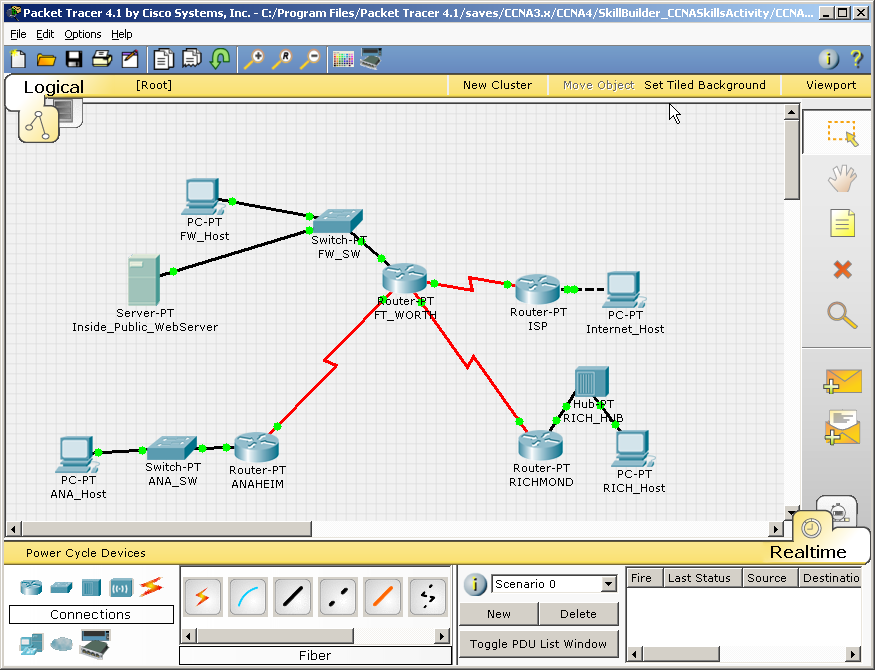
\includegraphics[width=12cm]{obrazky/packet-tracer}
\caption{Packet tracer}
\label{obr_packet-tracer}
\end{center}
\end{figure}



%------------------------------------------------------------------------------------------------------

\section{AdventNet Simulation Toolkit}

% AdventNet Simulation Toolkit 6
% AdventNet Simulation Toolkit 6 [7] je kompletný grafický softvérový simulátor
% zariadení a sietí s veľkou podporou viacerých protokolov, Cisco IOS zariadení a iných
% zariadení ako napr. rôzne Linux, či Windows 2000 servery. Tento simulátor je dostupný
% vo verzii nie len pre Windows, ale aj pre Linux a Solaris. Zo stránky sa dá po poskytnutí
% osobných údajov stiahnuť plne funkčná skúšobná verzia na 30 dní. Je síce limitovaná
% na maximálny počet 25 simulovaných prvkov, ale na začlenenie do tejto práce je postačujúca.

\uv{AdventNet Simulation Toolkit je kompletní grafický softwarový simulátor zařízení a sítí s velkou podporou mnohých protokolů, Cisco IOS zařízení a jiných zařízení jako např. různé Linux, či Windows 2000 servery.}\cite{resersni_bakalarka} Argumentem proti použití tohoto programu je především jeho cena, plná časově neomezená verze stojí od \$995 do \$14995 \footnote{k 23.5.2010}. K disposici je zkušební třicetidení verze.



%------------------------------------------------------------------------------------------------------

\section{Simulační software Omnet++}

\uv{Simulační systém OMNeT++ [11] je velmi propracovaný opensource nástroj pro simulaci prakticky čehokoliv. OMNeT++ je postaven na modulární architektuře, takže při správných knihovnách (modulech) může simulovat počítačovou síť. Systém dokáže simulovat Cisco IOS i počítač postavený na linuxu.}\cite{resersni_bakalarka}. Systém se však hodí spíše pro simulaci zatížení sítě a pro simulaci síťových protokolů. K výukovým účelům není příliš vhodný kvůli své složitosti.

Více se tímto simulátorem zabýval Bc. Jan Michek v~rámci své diplomové práce Emulátor počítačové sítě \cite{reserse:omnet_dp}.

% omnet
\begin{figure}[h]
\begin{center}
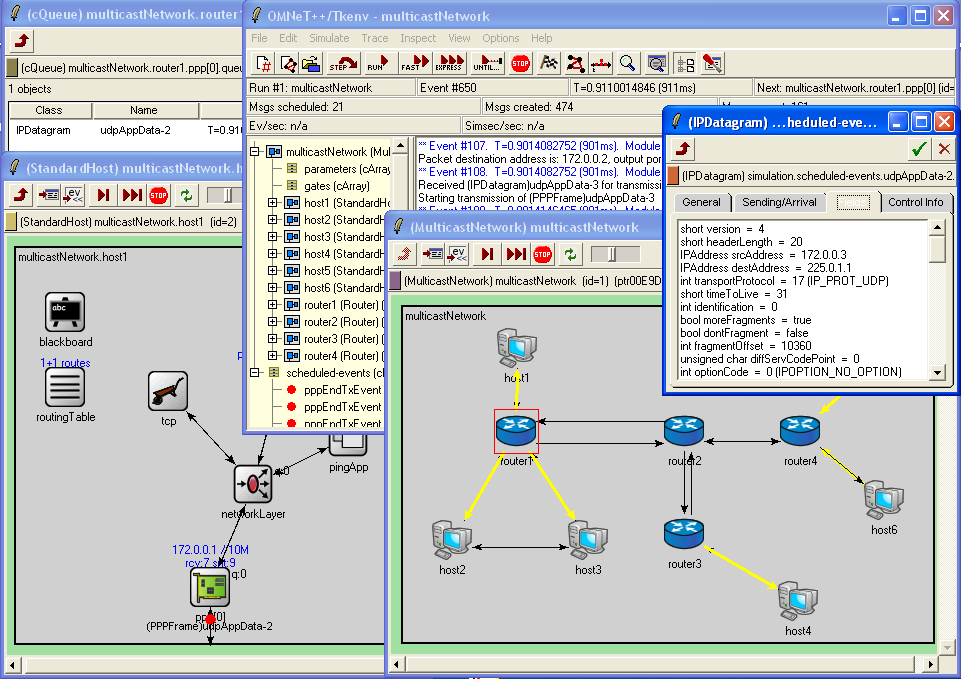
\includegraphics[width=12cm]{obrazky/omnet}
\caption{Omnet++}
\label{obr_omnet}
\end{center}
\end{figure}



%------------------------------------------------------------------------------------------------------

\section{Závěr}

Tvůrci simulačních programů dávají většinou přednost simulaci sítí založených na síťových prvcích ood firmy Cisco. Podporují-li i počítače s linuxem, ani o tom moc nepíší. Většina simulátorů je studentům nedostupná kvůli své ceně. Studenti předmětu PSI budou simulátor potřebovat pravděpodobně jen několikrát za semestr a je nesmyslné, aby si škola, nebo sami studenti kupovali kvůli několika použitím licenci.



\chapter{Analysa aplikace}

V této kapitole se zabývám analysou a návrhem aplikace jako celku. Shrnuji a analysuji požadavky, diskutuji zvolený jazyk a uživatelské rozhraní, navrhuji architekturu aplikace a odhaduji její náročnost. Analysa jednotlivých částí simulátoru je popisována společně s těmito částmi.


%-----------------------------------------------------------------------------------

\section{Požadavky na aplikaci}

Nejprve shrnu všechny požadavky na mojí aplikaci.

\subsection{Funkční požadavky}
\begin{enumerate}
 \item Vytvoření počítačové sítě založené na počítačích OS Linux.
 \item Aplikace umožňuje konfiguraci rozhraní pomocí příkazů ifconfig a ip addr.
 \item Aplikace obsahuje funkční směrování a umožňuje jeho nastavování pomocí příkazů route a ip route.
 \item Aplikace implementuje překlad adres
 \item Aplikace podporuje ukládání a načítání do/ze souboru.
 \item Pro ověření správnosti jsou implementovány příkazy ping a traceroute.
 \item K jednotlivým počítačům aplikace je možné se připojit pomocí telnetu.
 \item Pomocí telnetu bude možno se připojit zároveň k více virtuálním počítačům.
 \item Pomocí telnetu bude možno připojit se k jednomu počítači vícekrát najednou.
\end{enumerate}

\subsection{Nefunkční požadavky}
\begin{enumerate}
 \item Aplikace bude multiplatformní - alespoň pro operační systémy Windows a Linux
 \item Aplikace musí být spustitelná na běžném\footnote{Slovem \uv{běžné} se myslí v podstatě jakýkoliv počítač, na kterém je možné nainstalovat prostředí Javy - Java Runtime Environment} studentském počítači.
 \item Aplikace by měla být co nejvěrnější kopií reálného počítače s Linuxem.
\end{enumerate}



%-----------------------------------------------------------------------------------

\section{Analysa požadavků}


\subsection{Připojení pomocí telnetu}

Jedním z funkčních požadavků mé aplikace je možnost připojit se k jednotlivým virtuálním počítačům pomocí protokolu telnet. Tento požadavek vypadá jednoduše, pokud pod pojmem Telnet chápeme jednoduchý protokol na přenos textových dat. Takový protokol ovšem neumožňuje doplňování příkazů a jejich historii, což je pro práci s počítačem, byť virtuálním, obrovské omezení. Oproti tomu, implementovat telnet protokol, jako NVT\footnote{NVT – Network Virtual Terminal, česky: Síťový virtuální terminál; poskytuje standardní rozhraní příkazové řádky}, kde se posílá a potvrzuje každý napsaný znak, by překračovalo rozsah této bakalářské práce. Můj kolega nalezl program rlwrap, který poskytuje historii příkazů a jejich doplňování na straně klienta. Funguje v linuxu, na windowsu jen pod cygwinem. Toto druhé řešení bude o dost jednodušší a rozhodli jsme se ho realisovat, i když pro uživatele bude nevýhodou spouštění přes cygwin. I tak ovšem základní požadavek, že s aplikací bude možno komunikovat pomocí telnetu, zůstane zachován, uživatel ovšem přijde o komfort, který mu nabízí možnost doplňování, editace a historie příkazů. 


\subsection{Podobnost simulátoru se skutečným linuxem}

Aby byl simulátor využitelný pro výukové účely, musí být dostatečně podobný skutečnému linuxu, aby uživatel mohl věřit, že to, co funguje v simulátoru, bude fungovat i na skutečném linuxu a naopak. K tomu bude stačit implementovat jen ty příkazy, kterými se nastavují síťové parametry, a jen v takovém rozsahu, jaký je pro tyto výukové účely potřeba. Budu tedy implementovat příkazy \verb|ifconfig\verb|, \verb|route|, \verb|ping| a \verb|traceroute|, z příkazu \verb|ip| stačí implementovat jeho podpříkazy \verb|addr| a \verb|route|. Pro potřeby nastavení překladu adres je potřeba implementovat malou část příkazu \verb|iptables|. Aby uživatel mohl nastavovat některé hodnoty souborů v adresáři \verb|/proc|, implementuji ve velmi omezené míře i příkazy \verb|cat| a \verb|echo|, ovšem jen pro tyto soubory. Pro ukončení spojení bude implementován příkaz \verb|exit|. Pro potřeby simulátoru ale není potřeba implementovat kompletní příkazy \verb|ifconfig| nebo \verb|ip|, ale jen tu jejich část, kterou se nastavují parametry rozhraní, jako IP, maska a další. O ostatních parametrech pak vetšinou simulátor vypíše, že ve skutečnosti sice existují, ale simulátorem zatím nejsou podporované.


\subsection{Počet simulovaných počítačů}

Na laboratořích Y36PSI studenti konfigurují 4 počítače, náš simulátor by měl zvládnout simulovat síť o 10 počítačích. Více ani není potřeba, pro výukové účely studenti pravděpodobně nebudout konfigurovat více počítačů.



%-----------------------------------------------------------------------------------

\section{Programovací jazyk a uživatelské rozhraní}

\subsection{Programovací jazyk}
Aplikaci jsme se rozhodli programovat v programovacím jazyku Java z několika důvodů. Java je programovací jazyk, který nabízí velký programátorský komfort, stabilitu a zároveň možnost vytvořené aplikace používat pod různými operačními systémy, což je další z nefunkčních požadavků. Tento jazyk navíc disponuje hotovými knihovnami pro práci se sítí v balíčku java.net. Dalším důvodem je také to, že s programováním aplikací v Javě mám zatím asi největší zkušenosti.

\subsection{Uživatelské rozhraní}

Jak plyne ze zadání, uživatel se přihlašuje k jednotlivým virtuálním počítačům pomocí programu telnet, nemusím tedy vytvářet žádného speciálního klienta. S aplikací samotnou nebude uživatel nijak pracovat, jenom ji spustí se správným konfiguračním souborem a případně číslem výchozího portu, dále již bude nastavovat pouze jednotlivé virtuální počítače pomocí telnetu. Pro takovou aplikaci je nejlepším uživatelským rozhraním příkazová řádka, vytváření grafického uživatelského rozhraní by nemělo smysl.



%-----------------------------------------------------------------------------------

\section{Návrh architektury}

Aplikace se bude skládat ze dvou vrstev. Komunikační vrstva by měla zajišťovat síťovou komunikaci s klientem, tedy odesílání a přijímání textových dat. Z velké části bude převzata z jiné práce, kterou jsme kdysi dělali jako domácí úkol na předmět Y36PSI. Aplikační vrstva bude tvořena samotnou virtuální sítí. Tyto vrstvy však od sebe nebudou striktně odděleny. Nejprve si rozebereme druhou vrstvu.


\subsection{Virtuální síť}

Virtuální počítačová síť, kterou bude aplikace simulovat, má poskytovat především tyto funkcionality:
\begin{itemize}
 \item Možnost konfigurace jednotlivých síťových prvků.
 \item Posílání paketů mezi síťovými prvky.
\end{itemize}
Skutečná počítačová síť se skládá ze síťových prvků různých druhů. Stejně tak i virtuální síť se bude skládat ze síťových prvků, které budou interně reprezentovány objekty.

\subsubsection{Síťové prvky}

V laboratořích předmětu Y36PSI studenti nastavují pouze PC nebo směrovače na 3. (síťové) vrstvě ISO/OSI modelu\footnote{3. vrstva ISO modelu, tzv. síťová vrstva, zajišťuje spojení mezi jakýmikoliv 2 uzly sítě.}. Síťové prvky pracující na 2. vrstvě ISO/OSI modelu\footnote{2. vrstva ISO/OSI modelu, tzv. spojová nebo linková vrstva, zajišťuje spojení mezi dvěma sousedními systémy.}, switche a bridge se v laboratořích vůbec neuvažují. Proto i ve své práci uvažuji jediný druh síťových prvků - počítače s OS Linux.

\subsubsection{Posílání paketů}
Virtuální síť musí umět posílat virtuální pakety, aby uživatel pomocí příkazů \verb|ping| nebo \verb|traceroute| zjistil, jestli virtuální síť správně nakonfiguroval. Posílání paktů bude vnitřně realisováno vzájemným voláním metod virtuálních počítačů, které si mezi sebou budou předávat objekty typu paket. Tyto metody zřejmě bude vhodné rozdělit tak, aby odpovídaly jednotlivým vrstvám ISO/OSI modelu.


\subsection{Komunikační vrstva}
Komunikační vrstva simulátoru bude zajišťovat spojení aplikace s klientem. Z tohoto pohledu bude simulátor klasickým síťovým serverem, který poslouchá na několika portech, přijímá spojení a zpracovává je. Uživatel bude po síti konfigurovat jednotlivé virtuální počítače, proto každý virtuální počítač musí poslouchat na jednom portu. Pro obsluhu této komunikace bude vytvořeno několik tříd. Aby mohl simulátor poslouchat na více portech najednou, bude nutné vytvořit více vláken, každý virtuální počítač tedy poběží v samostatném vláknu. Jak plyne z posledního funkčního požadavku, musí jeden virtuální počítač umět zpracovat i více spojení najednou, jako i na reálný linuxový počítač je možné se připojit k několika jeho terminálům pomocí protokolu ssh nebo telnet. Proto bude nutné, aby vlákno, které poslouchá na portu, pro příchozí spojení vytvořilo jiné vlákno, které spojení obslouží, a samo dále poslouchalo na určeném portu. 



%-----------------------------------------------------------------------------------

\section{Odhad náročnosti aplikace}

Aplikace nebude mít žádné uživatelské rozhraní, nebude přistupovat do žádné database a její datové struktury budou pravděpodobně poměrně jednoduché. Proto pro virtuální síť o deseti počítačích by spotřeba paměti by neměla překročit požadavky pro běžné aplikace v~Javě. Simulátor by mohl potřebovat odhadem 10-30MB bez načteného prostředí JRE.



%-----------------------------------------------------------------------------------

\section{Odhad složitosti práce a jejího průběhu}

Celý projekt by měl být v~rozsahu zhruba 10000 řádků kódu a měl by být dokončen do konce dubna 2010.


\chapter{Implementace virtuální sítě}

V této kapitole se zabývám analysou a implementací jednotlivých částí aplikace. Rozebírám zde nejprve analýzu a implementaci třídy \verb|IpAdresa|, dále implementaci virtuálního počítače, analýzu a implementaci routovací tabulky a analýsu a implementaci posílání paketů. Nezabývám se zde analysou a implementací jednotlivých příkazů, vzhledem k rozsáhlosti tohoto tématu jsem ho vyčlenil do zvláštní kapitoly, která následuje za touto kapitolou.



%----------------------------------

\section{IP adresa}

Třída \verb|IpAdresa| je sice jen jednou z mnoha tříd, vzhledem k jejímu významu ji ale v následujících odstavcích popíšu podrobněji.


\subsection{Analýza}

Protože simulátor se zabývá především simulací síťové vrstvy ISO/OSI modelu, je síťová adresa počítače, tzv. IP adresa velmi často používanou datovou strukturou, pro kterou se jistě vyplatí mít speciální třídu. Ta se v v aplikaci jmenuje \verb|IpAdresa| a patří do balíčku \verb|datoveStruktury|. Je používána jako parametr síťového rozhraní, jako prefix v routovací tabulce, jako zdrojová a cílová adresa v paketech. Při bližším pohledu je zřejmé, že kontext jejího použítí se v těchto případech částečně liší. Například pro posílání paketů je nutné, aby paket obsahoval zdrojovou a cílovou adresu i s portem. Port by samozřejmě nemusel být součástí adresy, ukázalo se to však jako jednoduší a pro posílání paketů přehlednější možnost. Pro IP adresu jako parametr rozhraní je naopak port zcela nesmyslný parametr, nutně ale potřebuje parametr pro síťovou masku, která je naproti tomu nesmyslná pro posílání paketů. Paket posílám na IP adresu, ne na adresu s maskou.


\subsection{Vnitřní reprezentace}

Přes tyto rozdíly jsem se rozhodl vytvořit pro IP adresu jednu třídu, která má parametry \verb|adresa|, \verb|maska| a \verb|port|, přičemž pro danou situaci nepotřebné parametry prostě ignoruji. Protože Java neobsahuje žádný 32-bitový bezeznaménkový datový typ, jsou parametry adresa a maska vnitřně reprezentovány 32-bitovým integerem, který ale obsahuje bity skutečné adresy, jeho číselná hodnota není důležitá. Operace s nimi se provádí především pomocí bitových operátorů. Parametr port je normální integer.


\subsection{Veřejné metody}

\verb|IpAdresa| má konstruktory, aby ji bylo možné vytvořit ze \verb|Stringu|, s maskou zadanou jako \verb|String|, \verb|Integer| nebo v jednou řetězci s adresou. Adresu je možné převést na String nebo porovnat s jinou adresou mnoha různými způsoby, například jen podle adresy, adresy s portem,  adresy s maskou nebo čísla sítě. \verb|IpAdresa| umí vrátit své číslo sítě nebo broadcast jako jinou \verb|IpAdresu|. O těchto metodách se zde nerozepisuji podrobně, v kódu jsou dobře okomentované.



%----------------------------------

\section{Virtuální počítač}

Virtuální počítač je základním stavebním prvkem naší aplikace. Pracuje na obou jejích vrstvách. Na vrstvě komunikační přijímá a zpracovává příchozí spojení, na aplikační vrstvě, tj. na vrstvě virtuální sítě přijímá, posílá a přeposílá pakety. Posíláním paketů se zabývám až v posledním odstavci této kapitoly, zde proberu komunikační vrstvu počítače a jeho rozhraní.

Protože linuxový a ciscový počítač, který dělal kolega, mají mnoho společného, vytvořil jsem abstraktní třídu \verb|AbstraktniPocitac|, který je předkem počítačů obou typů. Třída \verb|LinuxPocitac| má ale jen jednu metodu, která se týká posílání paketů, proto ji zatím ignoruji.

Všechny virtuální počítače jsou vytvářeny v rámci inicialisace aplikace dle konfiguračního souboru na začátku jejícho běhu, za chodu aplikace není již možné další počítač přidat nebo nějaký odebrat. O komunikaci s uživateli se stará třída Komunikace. Počítač si drží seznam svých síťových rozhraní, svoji routovací tabulku a natovací tabulku. Má jediný konstruktor, kde je mu zadáno jméno (pro přehlednost) a port, na kterém má být dostupný pro uživatele.


\subsection{Komunikace s počítačem}

V konstruktoru abstraktního počítače je volán konstruktor jeho parametru třídy \verb|Komunikace|. Tato třída se stará o veškerou komunikaci s uživatelem. Je potomkem třídy Thread. Běží ve vlastním vlákně, které se startuje v jejím konstruktoru, a poslouchá na portu, který jí byl zadán. Pro každé nové příchozí spojení vytvoří instanci třídy konsole, která spojení obslouží, aby komunikce mohla dále poslouchat na portu a zpracovávat další spojení. Třída Konsole je také potomkem třídy Thread. Obsluhuje jedno telnetové připojení. Drží si instanci třídy ParserPrikazu z balíčku Prikazy (o něm v následující kapitole). Přijímá textová data od uživatele až po enter (sekvence \verb|\r\n|), tedy vlastně načítá data po řádcích. Každý řádek, který ji uživatel pošle, předá parseru na zpracování a pak sama pošle uživateli prompt. Parseru poskytuje metody pro posílání textových dat uživateli. Pro uživatele tak komunikace s touto Konsoli vypada stejně jako práce s příkazovou řádkou na skoutečném počítači.


\subsection{Síťové rozhraní}

%v tomhle adstavci by chtela dodelat ta footnote
Z hlediska infrastruktury sítě jsou základními prvky počítače jeho síťová rozhraní. Ty si počítač drží v seznamu. Jsou vytvořeny při parsovaní konfiguračního souboru a během běhu aplikace je nelze nijak měnit, přidávat nebo mazat. Třída \verb|SitoveRozhrani| má svoje jméno a fysickou (mac) adresu. Protože v naší aplikaci není implementován ARP\footnote{Address Resolution Protocol se v počítačových sítích s IP protokolem používá k získání ethernetové MAC adresy sousedního stroje z jeho IP adresy. Používá se v situaci, kdy je třeba odeslat IP datagram na adresu ležící ve stejné podsíti jako odesílatel. Data se tedy mají poslat přímo adresátovi, u něhož však odesilatel zná pouze IP adresu. Pro odeslání prostřednictvím např. Ethernetu ale potřebuje znát cílovou ethernetovou adresu.\cite{wiki:arp}} protokol, mac adresa nemá jiný význam, než že je vypisována příkazy jako např. \verb|ifconfig|.

Skutečné síťové rozhraní může mít více adres. Tato možnost však není v předmětu PSI využívána, proto jsem ji neimplementoval. Znamenalo by to totiž poměrně velké problémy v posílání paketů. Musel bych složitě zjišťovat, kdy se paket odešle s jakou síťovou adresou, pokud je jich na daném rozhraní více. Pro potřeby statického překladu adres (NAT) především na ciscovém routeru je ale nutné mít na rozhraní více adres\footnote{Více o překladu adres v bakalářské práci mého kolegy Stanislava Řeháka}. Proto má třída \verb|SitoveRozhrani| seznam IP adres, ale jeho první adresa je privilegovaná. Každý paket, který je přes dané rozhraní posílán, má jako odchozí adresu adresu právě první tohoto rozhraní. První adresa je vždy nastave, není-li nakonfigurována, je nastavena na \verb|null|. Tuto jedinou adresu lze nastavovat a vypisovat. Ostatní adresy jsou přidávány jen pro potřeby statického natování. Pokud rozhraní nemá nastavenou žádnou adresu, je první (privilegovaná) adresa \verb|null|.



%----------------------------------

\section{Routovací tabulka}

% OSNOVA
% - co to je, struktura týhle části
% - použití pro cisco
% Analysa
% 	Struktura tabulky
% 	Adresát - vysvětlit, jak to funguje
% 	Příznaky
% 	Přidávání záznamů a jejich řazení
% 	Mazání záznamů
% 	Použití při směrování
% Implementace
% 	Vnitřní reprezentace (struktura)
% 	Přidávání, mazaní a řazení záznamů - jednotlivý metody, metoda pro parser konfiguráku
% 	Použití při směrování - metody

Počítače směrují pakety podle tzv. routovací, neboli směrovací, tabulky. \uv{Routovací tabulka je datový soubor uložený v RAM paměti, který je používán k uchovávání informací ohledně přímo připojených i vzdáleně připojených sítích. Její obsah napovídá routeru, kterým rozhraním je možno nejoptimálněji dosáhnout cílové sítě.}\cite{owebu:routovaci_tabulka}. V této části se zabývám nejprve analýzou routovací tabulky na skutečném linuxu a potom popisuji její implementaci v simulátoru.

Třída \verb|RoutovaciTabulka| měla být původně stejně použitelná pro linux i pro cisco. Až po tom, co jsem jí implementoval, kolega zjistil, že pro potřeby Cisca není tato třída bez úprav použitelná. Proto implementoval třídu \verb|CiscoWrapper|, která obaluje třídu \verb|RoutovaciTabulka| a dodává jí funkce potřebné pro cisco. To však není obsahem mojí práce.


\subsection{Analýza routovací tabulky na skutečném počítači}

\subsubsection{Struktura tabulky}

V řádcích routovací tabulky jsou záznamy pro jednotlivé sítě. Každý záznam má tyto parametry:
\begin{itemize}
\item adresát - IP adresa s maskou, pro kterou je tento záznam platný
\item brána - IP adresa počítače, na který se má paket poslat. Tento sloupec nemusí být vždy vyplněn.
\item příznaky - O těch více píšu v samostatné části.
\item metrika - Jedno z kriterií priority.
\item rozhraní - Rozhraní, přes které se paket posílá.
\end{itemize}
Parametr metrika není pro výukové účely potřeba, proto se jím již dále nezabývám.

Pro lepší představu zde vkládám routovací tabulku tak, jak je vypsána příkazem \verb|route -n|:
\begin{verbatim}
Adresát         Brána           Maska           Přízn Metrik Odkaz  Užt Rozhraní
147.32.125.128  0.0.0.0         255.255.255.128 U     1      0        0 eth0
169.254.0.0     0.0.0.0         255.255.0.0     U     1000   0        0 eth0
0.0.0.0         147.32.125.129  0.0.0.0         UG    0      0        0 eth0
\end{verbatim}

\subsubsection{Adresát}

V hořejším výpisu tabulky pomocí příkazu \verb|route| se adresáta týkají 2 sloupce, sloupec Adresát a sloupec Maska, ve kterém jsou vypsány masky k IP adresám uvedeným ve sloupci Adresát. Tyto IP adresy s maskami jsou vždy číslem sítě a reprezentují všechny adresy, které do této sítě patří. Tak například adresát 0.0.0.0/0 reprezentuje úplně všechny IP adresy, adresát 147.32.125.128/25 reprezentuje adresy v rozmezí 147.32.125.128 až 147.32.125.255, adresát 1.1.1.1/32 reprezentuje jedinou adresu 1.1.1.1 a adresát 192.168.1.0/24 reprezentuje všechny adresy, které začínají byty 192.168.1.x. Adresáta 147.32.125.128/24 nelze zadat, protože číslo této sítě je 147.32.125.0/24.

\subsubsection{Příznaky}\label{routTabulka-priznaky}

Záznam routovací tabulky má několik příznaků. Má vždy minimálně jeden příznak, může mít ale všechny 3 příznaky najednou. Zde je jejich popis:
\begin{itemize}
\item Příznak \verb|U| znamená, že záznam obsahuje rozhraní. Protože záznam bez vyplněného rozhraní není možné zadat, má tento příznak každý záznam.
\item Záznam má příznak \verb|G|, jestliže je vyplněn sloupec brána.
\item Příznak H znamená, že adresátem daného záznamu je jeden počítač, tzn. adresát má masku 255.255.255.255.
\end{itemize}
Příznak \verb|H| jen informuje, že adresát není sítí ale jediným počítačem, není tedy nijak důležitý. Podle příznaků existují 2 typy záznamů, záznamy s příznakem \verb|U| a záznamy s příznakem \verb|UG|. Tyto typy se liší jak při přidávání nových záznamů do routovací tabulky, tak při posílání paketu podle tohoto záznamu. Posílá-li počítač paket podle záznamu U, není z tohoto záznamu zřejmé, jakému sousednímu počítači (na linkové vrstvě) se má paket poslat. Počítač se tedy pokusí poslat paket přímo na cílovou IP adresu uvedenou v paketu. Posílá-li se paket podle záznamu UG, posílá se na adresu brány uvedenou v záznamu. Více se této problematice věnuji v kapitole o posílání paketů.

\subsubsection{Přidávání záznamů a jejich řazení}

Routovací tabulka nesmí obsahovat 2 stejné záznamy. Za stejné záznamy se považují záznamy, které mají stejného adresáta včetně masky, stejné rozhraní a stejnou bránu.

Záznam typu \verb|U| lze přidat vždycky. Záznam typu \verb|UG| lze přidat jen pod podmínkou, že jeho brána je v okomžiku přidání dosažitelná záznamem typu \verb|U|. Tím je možné dosáhnout zajímaveho chování: Když do routovací tabulky přidám defaultní routu \footnote{Defaultní routa je záznam platný pro ccelý internet, jeho adresátem je 0.0.0.0/0} záznamu typu U, můžu pak přidat routu na jakoukoliv síť v internetu se záznamem UG. Když potom smažu původní defaultní routu, můžu posílat pakety pouze na tu síť s příznakem \verb|UG| a na počítač v mé síti paket neodešlu. Zde uvádím příklad:
\begin{verbatim}
root: /home/neiss# route add default eth0
root: /home/neiss# route add -net 89.190.94.0/24 gw 89.190.94.1
root: /home/neiss# route del default
root: /home/neiss# route
Směrovací tabulka v jádru pro IP
Adresát         Brána           Maska           Přízn Metrik Odkaz  Užt Rozhraní
89.190.94.0     89.190.94.1     255.255.255.0   UG    0      0        0 eth0
root: /home/neiss# ping -c1 89.190.94.58
PING 89.190.94.58 (89.190.94.58) 56(84) bytes of data.
64 bytes from 89.190.94.58: icmp_seq=1 ttl=53 time=14.1 ms

--- 89.190.94.58 ping statistics ---
1 packets transmitted, 1 received, 0% packet loss, time 0ms
rtt min/avg/max/mdev = 14.141/14.141/14.141/0.000 ms
root: /home/neiss# ping -c1 147.32.125.129				# toto je adresa brány, přes kterou šel minulý paket
connect: Network is unreachable
\end{verbatim}
Tento pokus funguje ale jen tehdy, pokud moje brána, v tomto případě 147.32.125.129 je cisco (viz část o posílání paketů).

Záznamy se v tabulce řadí podle masky adresáta. Nahoře jsou záznamy s nejdelší maskou, tzn. záznamy nejkonkrétnější. Pokud vkládám více záznamů se stejnou maskou, chová se routovací tabulka naprosto nepředvídatelně, což je vidět na následujícím příkladě:
\begin{verbatim}
node-4:/home/dsn# route add -net 1.1.5.0/25 dev eth0
node-4:/home/dsn# route add -net 1.1.6.0/25 dev eth0
node-4:/home/dsn# route add -net 1.1.7.0/25 dev eth0
node-4:/home/dsn# route add -net 1.1.8.0/25 dev eth0
node-4:/home/dsn# route add -net 1.1.9.0/25 dev eth0
node-4:/home/dsn# route add -net 1.1.10.0/25 dev eth0
node-4:/home/dsn# route add -net 1.1.11.0/25 dev eth0
node-4:/home/dsn# route add -net 1.1.12.0/25 dev eth0
node-4:/home/dsn# route add -net 1.1.13.0/25 dev eth0
node-4:/home/dsn# route add -net 1.1.14.0/25 dev eth0
node-4:/home/dsn# route add -net 1.1.15.0/25 dev eth0
node-4:/home/dsn# route
Kernel IP routing table
Destination     Gateway         Genmask         Flags Metric Ref    Use Iface
1.1.10.0        *               255.255.255.128 U     0      0        0 eth0
1.1.11.0        *               255.255.255.128 U     0      0        0 eth0
1.1.8.0         *               255.255.255.128 U     0      0        0 eth0
1.1.9.0         *               255.255.255.128 U     0      0        0 eth0
1.1.14.0        *               255.255.255.128 U     0      0        0 eth0
1.1.6.0         *               255.255.255.128 U     0      0        0 eth0
1.1.15.0        *               255.255.255.128 U     0      0        0 eth0
1.1.7.0         *               255.255.255.128 U     0      0        0 eth0
1.1.12.0        *               255.255.255.128 U     0      0        0 eth0
1.1.13.0        *               255.255.255.128 U     0      0        0 eth0
1.1.5.0         *               255.255.255.128 U     0      0        0 eth0
\end{verbatim}
Podle jakého algoritmu jsou nové záznamy zařazovány je mi opravdu záhadou.

\subsubsection{Mazání záznamů}

Smazat je možno jakýkoliv záznam tabulky. Pro mazání záznamů je potřeba zadat správně minimálně adresáta záznamu. Pokud pak existuje více záznamů se zadanými parametry, smaže se první z nich. Smazání jakéhokoliv záznamu nijak neovlivní ostatní záznamy.

\subsubsection{Použití pro směrování}\label{routTabulka_pouzitiPriSmerovani}

Ke směrování paketu se použije první záznam odpovídající cílové adrese. To znamená, že bude-li v routovací tabulce dané adrese odpovídat více záznamů, použije se ten nejvíce nahoře. Protože záznamy jsou řazeny podle délky síťové masky, je vrácený záznam ten nejkonkrétnější.


\subsection{Implementace routovací tabulky v simulátoru}

Routovací tabulka je imlementována třídou \verb|RoutovaciTabulka|, jejíž odkaz si drží \verb|AbstraktniPocitac| a podle ní směruje pakety.

\subsubsection{Vnitřní reprezentace}

Tabulka je vnitřně reprezentována seznamem objektů typu \verb|Zaznam|, který reprezentuje jeden záznam, tj. řádek tabulky. Záznam routovací tabulky má v simulátoru jen tyto parametry: adresát, brána a rozhraní, které fungují tak, jak bylo popsáno v odstavci o analyse. Parametry adresát a brána jsou typu \verb|IpAdresa|, parametr rozhraní je typu \verb|SitoveRozhrani|. Parametr záznamy není vůbec potřeba. Příznak \verb|U| musí mít záznam vždy, příznak \verb|H| má právě tehdy, když adresát má masku 255.255.255.255, a příznak \verb|U| má záznam právě tehdy, když má vyplněnou položku brána, proto ani ten není potřeba.

\subsubsection{Přidávání, mazání a řazení záznamů}

Záznamy jsou přidávány pomocí 2 metod se stejným názvem \verb|pridejZaznam| ale jinými parametry. Jedna přidává záznam typu \verb|U|, druhá, která má navíc paramatr brána, záznam typu \verb|UG|. U obou se kontroluje, jestli tabulka již stejný záznam neobsahuje, u té druhé se navíc kontroluje dosažitelnost brány, jak bylo popsáno v analýze.

Záznamy se samozřejmě řadí podle masky jako v reálné tabulce, záznamy se stejnou maskou se ale vloží vždy nad původní záznam. Tak jsou novější záznamy vždy nahoře. Zmatečné řazení reálné tabulky jsem samozřejmě neimplementoval.

Pro mazání má \verb|RoutovaciTabulka| metodu \verb|SmazZaznam|, funguje stejně jako na reálném počítači.

Navíc obsahuje \verb|RoutovaciTabulka| ještě metodu \verb|pridejZaznamBezKontrol|, která je využívána při vytváření počítače z konfiguračního souboru, jinde se nepoužívá.

\subsubsection{Použití při směrování}

K samotnému směrování slouží metoda \verb|najdiSpravnejZaznam|, která vrací celý řádek routovací tabulky. Funguje stejně jako na reálném počítači.



%----------------------------------

\section{Posílání paketů}

% Osnova sekce:
% - popsat, k čemu se u nás paety posílaj
% - popsat strukturu týhle části - DODĚLAT !!!
% Referenční model ISO/OSI
% 	- popsat vrstvy skutečný sítě, který se nás týkaj, zabalování rámců, atd
% 	Datové bloky
% implementace našeho paketu
% Chování reálného počítače při posílání paketů
% 	Trensportní vrstva - icmp
% 	Síťová vrstava - IP
% 		ip_forward
% 		Směrování
% 		ttl
% 		Next hop
% 	Linková vrstva - ethernet
% 	Zajímavosti - DODĚLAT!!!
% popsat implementaci
% 	- rozdělení do vrstev
% 	jednotlivý metody

Posílání paketů v naší aplikaci slouží k tomu, aby uživatel pomocí příkazů \verb|ping| a \verb|traceroute| mohl ověřit, zda síť správně nakonfiguroval. Bez této části by naší aplikaci nebylo možné nazvat síťovým simulátorem.


\subsection{Referenční model ISO/OSI}

\uv{Referenční model ISO/OSI vypracovala organizace ISO jako hlavní část snahy o standardizaci počítačových sítí.}\cite{wiki:referencni_model}. Dle tohoto modelu probíhá síťová komunikace v sedmi vrstvách, z níž každá poskytuje přesně definované funkce a komunikuje jen s vrstvou sousední. Každá vrstva má svůj formát přenášených dat, obyčejně dělených do bloků. Pro moji aplikaci jsou důležité vrstvy 2 - 4, tzn. spojová, síťová a transportní vrstva.

\subsubsection{Spojová vrstva}

Spojová nebo linková vrstva\footnote{Více v \cite{wiki:linkova_vrstva}} \uv{poskytuje spojení mezi dvěma sousedními systémy.}\cite{wiki:referencni_model}. Tuto vrstvu zajišťuje na skutečné síti v laboratoři technologie Ethernet\cite{wiki:ethernet}, ke zjištění fysické adresy sousedního systému se používá protokol ARP\cite{wiki:arp}. Sousednímy systémy se zde rozumí počítače zapojené do stejné sítě. Blok dat na linkové vrstvě se nazývá rámec. Vzhledem k tomu, že simulátor neobsahuje žádné switche, zajištuje tato vrstva v naší aplikaci spojení mezi 2 počítači propojenými kabelem.

\subsubsection{Síťová vrstva}

Síťová vrstva \uv{se stará o směrování v síti a síťové adresování. Poskytuje spojení mezi systémy, které spolu přímo nesousedí.}\cite{wiki:referencni_model} Zajišťuje spojení meze jakýmikoliv dvěma uzly sítě. Obyčejně je realizována protokolem IP\footnote{Internet Protocol}. Blok dat na síťové vrstvě se nazává paket.

\subsubsection{Transportní vrstva}

Transportní vrstva \uv{zajišťuje přenos dat mezi koncovými uzly}\cite{wiki:referencni_model}. Pro potřeby příkazů ping a traceroute je tato vrstva realisována protokolem ICMP\footnote{Internet Control Message Protocol, více v \cite{wiki:icmp}}. Blok dat se v transportní vrstvě nazývá datagram.

\subsubsection{Datové bloky}\label{datove_bloky}

Datový blok jakékoliv vrstvy se skládá z hlavičky, která obsahuje režijní informace té vrstvy, a z datové části, která obsahuje samotná data, ale i hlavičky vyšších vrstev. Tak například datagram protokolu ICMP je obalen hlavičkou IP na síťové vrstvě a hlavičkou protokolu Ethernet na spojové vrstvě.


\subsection{Implementace třídy Paket}
Pro můj síťový simulátor by bylo nesmyslné implementovat posílání paketů včetně jejich zabalování do datových bloku ruzných vrstev, tak jak je to popsáno v předchozím odstavci \ref{datove_bloky}. Proto jsem vytvořil třídu \verb|Paket|, která obsahuje všechny potřebné informace z datových bloků všech tří vrstev. \verb|Paket| má parametry síťové vrstvy, jako zdrojovou a cílovou adresu a \verb|ttl|, a parametry transportní vrstvy, jako typ a kód protokolu ICMP. Pro snadnější implementaci příkazu ping má parametr \verb|cas|, kam se ukládá náhodně generovaný čas běhu paketu, který vypisuje příkaz ping. Protože na jednom virtuálním počítači může běžet více příkazů \verb|ping| najednou, nese paket i odkaz na příkaz, který ho poslal, aby ho tento příkaz mohl také po jeho návratu zpracovat.

Typy a kódy ICMP paketů jsou označeny stejně jako ve skutečnosti:
\begin{itemize}
\item typ 0 - ozvěna (icmp reply) - odpověď na požadavek icmp request
\item typ 3 - vyslaný paket nemohl být doručen
\item typ 8 - žádost o ozvěnu (icmp request)
\begin{itemize}
\item kód 0 - network unreachable (nedosažitelná síť)
\item kód 1 - host unreachable (nedosažitelná adresa)
\end{itemize}
\item typ 11 - \verb|ttl| vypršelo
\end{itemize}


\subsection{Chování reálného počítače při posílání paketů}

\subsubsection{Transportní vrstva - protokol ICMP}

V souboru \verb|/proc/sys/net/ipv4/icmp_echo_ignore_all| je nastaveno, jestli počítač odpovídá na dotazy icmp reply. Pokud je v tomto souboru \verb|0|, počítač na dotazy odpovídá. Toto je defaultní nastavení, proto jsem v simulátoru tento problém vůbec neřešil a počítač odpovídá na icmp request vždy.

\subsubsection{Síťová vrstva - protokol IP}

\paragraph{Přeposílání paketů}
Počítač preposílá pakety jenom tehdy, pokud je v souboru \verb|/proc/sys/net/ipv4/ip_forward| jednička, jinak ne. Toto nastavení ale již není defaultní, proto ho musím v simulátoru implementovat. Proměnná \verb|ip_forward| je parametrem virtuálního počítače a je nastavována pomocí příkazu \verb|echo|.
\paragraph{Směrování paketů}
Pakety jsou směrovány podle routovací tabulky, kde se vybere první záznam odpovídající cílové adrese paketu, jak je popsáno v \ref{routTabulka_pouzitiPriSmerovani}. Pokud v routovací tabulce nebyl nalezen žádný záznam pro cílovou adresu paketu, pošle se na jeho zdrojovou adresu paket \verb|icmp_net_unreachable|\footnote{Tj ICMP paket typu 3 kódu 0}.
\paragraph{ttl}
Každý prvek, který pracuje i na síťové vrstvě sníží procházejícím paketům hodnotu \verb|ttl|. Pokud po tomto snížení dosáhne hodnota \verb|ttl| nuly, pošle počítač na zdrojovou adresu paketu zprávu \verb|icmp_ttl_exceeded|\footnote{Tj. icmp paket typu 11}.
\paragraph{Next hop}
Předtím než síťová vrstva předá odeslání paketu linkové vrstvě, musí pro tento paket zjistit tzv. next hop, neboli sousední adresu. \uv{Next hop je sousední směrovač, na který je paket poslán nebo přeposlán z daného směrovače na své cestě k cíli.}\cite{next_hop} Tato adresa je velmi důležitá pro linkovou vrstvu, která paket posílá právě na tuto adresu. Pokud je paket směrován podle záznamu typu \verb|UG| (viz \ref{routTabulka-priznaky}), je adresa next hop uvedena ve sloupci brána routovací tabulky. Pokud je paket směrován podle záznamu typu \verb|U|, je adresa next hop cílová adresa paketu. Podle routovací tabulky
\begin{verbatim}
Adresát         Brána           Maska           Přízn Metrika  Rozhraní
147.32.125.128  0.0.0.0         255.255.255.128 U     0       eth0
0.0.0.0         147.32.125.129  0.0.0.0         UG    0       eth0
\end{verbatim}
je pro pakety směrované podle prvního záznamu next hop rovná jejich cílové adrese. Pro pakety směrované podle druhého záznamu je next hop \verb|147.32.125.128|. Záznamy typu \verb|U| jsou tak používány pro počítače v mé síti, které jsou dosažitelné přímo bez jakéhokoliv mezilehlého směrovače. Záznamy \verb|UG| jsou používány pro počítače, na které je paket posílán přes jeden nebo více směrovačů.

\subsubsection{Linková vrstva}\label{skutecna_linkova_vrstva}

Na linkové vrstvě se rámce přeposílají jen mezi sousedními počítači. Běžně ji zajištuje protokol ethernet. IP adresu sousedního počítače, na kterou má rámec poslat, dostane od síťové vrstvy, musí ji přeložit na fysickou (MAC\footnote{Media Access Control}) adresu, což dělá protokolem ARP. Protokol ARP vyšle ethernetový rámec na všechny okolní počítače žádost, která obsahuje zadanou IP adresu. Pokud některý z počítačů má tokovou IP adresu, původnímu počítači pošle zpátky svoji fysickou adresu a ten pak může odeslat paket. Aby počítač nemusel fysickou adresu zjišťovat při odesílání každého rámce, ukládá si v datové struktuře nazvané ARP tabulka záznamy s IP adresami, které již dříve překládal.

Pokud počítač nemůže linkovou vrstvou odeslat rámec (paket), například proto, že počítač s takovou adresou na síti neexistuje,  pošle původnímu odesílateli ICMP paket \verb|net unreachable|\footnote{Tj ICMP paket typu 3 kódu 1}.

% ethernetový problémy na ciscu:
Počítač s operačním systémem linux odpovídá na ARP dotazy jen tehdy, když má požadovanou IP adresu nastavenou na svém rozhraní. V tom se liší od Cisca, které na ARP dotaz odpoví i v případě, že adresu na svém rozhraní nemá, ale ví, kam má paket dále směřoav, tzn. má pro požadovanou adresu záznam v routovací tabulce, a naopak na ARP dotaz neodpoví v případě, že nemá v routovací tabulce záznam pro IP adresu, odkud dotaz přišel. Pro lepší pochopení přepisuji podmínku ještě v jazyce booleanovských výrazů v javě:\\
Cisco odpoví na ARP dotaz právě tehdy, když:\\
Má záznam v routovací tabulce pro počítač, který ARP dotaz posílá \verb|&&| (Má nastavenou požadovanou IP adresu \verb|nebo| Má záznam v routovací tabulce pro cílovou adresu posílaného paketu)


\subsection{Implementace v simulátoru}

Pakety jsou mezi počítači posílány vzájemným voláním metod, které si mezi sebou předávají objekt typu \verb|Paket|. Všechny tyto metody jsou ve třídě \verb|AbstraktniPocitac|, protože to jsou právě virtuální počítače, které si mezi sebou pakety posílají. Jen metoda \verb|prijmiEthernetove| je sice v \verb|AbstraktniPocitac| zadeklarována a implementována v jeho potomcích.


Metody virtuálního počítače pro posílání paketů jsem bylo rozumné implementovat dle vrstev. Je to přehlednější, než kdybych měl jednu metodu pro přijmutí paketu a je to dobré i vzhledem k tomu, že linux a cisco se v některých případech liší a to jen na některých vrstvách. Metody jedné vrstvy tak volají jen metody vrstvy sousední, jako na reálné síti jedna vrstva komunikuje jen s vrstvami sousedními.

\subsubsection{Linková vrstva}

ARP protokol na zjišťování fysických adres nemusel být implementován, protože v síti nejsou žádné switche a v linkové vrstvě tak není potřeba žádné směrování. Aby ale byly splněny podmínky doručení nebo nedoručení paketu uvedené v \ref{skutecna_linkova_vrstva}, byly vytvořeny metody \verb|odesliEthernetove| a \verb|prijmiEthernetove|, které si mezi sebou předávají pakety tak, aby byly tyto podmínky splněny. Metoda \verb|prijmiEthernetove| na linuxu nepřijme paket, pokud nesouhlasí očekávaná IP adresa, jako kdyby neodpověděla na ARP dotaz.

\subsubsection{Síťová vrstva}

Na síťové vrstvě si pakety předávají metody \verb|odesliNovejPaket|, \verb|preposliPaket| a \verb|prijmiPaket|. Tyto metody směrují pakety a provádí překlad adres.

\subsubsection{Transportní vrstva}

Do transportní vrstvy patří více metod, které slouží především k posílání různých typů ICMP paketů.
  
  


\chapter{Implementace příkazů}

V této kapitole popisuji analýzu a realizaci linuxových příkazů, které jsou v simulátoru implementovány. Příkazy jsou nejrozsáhlejší částí mojí práce na simulátoru a nutno dodat, že také tou nejméně zábavnou. U každého příkazu jsem nejprve musel složitě zjišťovat, jak funguje a jak se chová v případě zadání nestandartních parametrů. Parsování příkazů bylo prací pořád stejnou a nezábavnou. 

V této kapitole nejprve popisuji zpracování příkazové řádky, pak obecné principy pro zpracování všech příkazů a nakonec popisuji analýzu a implementaci konkrétních příkazů.



%------------------------------------------------------------------------------------------------------

\section{Popis zpracování příkazové řádky}

Příkazovou řádku virtuálního počítače obsluhuje třída \verb|Konsole| (více v \ref{impl_komunikacni_vrstva}). Ta načítá textová data posílaná uživatelem až do sekvence \verb|\r\n|, kdy načítání zastaví a načtený řádek předá svému parseru. Každá \verb|Konsole| má svůj vlastní parser příkazů, který zpracovává jen jí poslané řádky a na ně odpovídá. \verb|Konsole| zavolá jeho metodu \verb|zpracujRadek|, která řádek \uv{rozseká} na jedotlivá slova a pak podle prvního slova, které by mělo být názvem příkazu, spustí odpovídající příkaz. Příkazům \verb|Konsole| poskytuje metody \verb|posliRadek| a \verb|posli|, pomocí kterých příkazy vypisují svůj výstup uživateli do konzole.

Architektura tříd pro zpracování příkazové řádky je celkem složitá, jak je vidět na obrázku \ref{obr_prikazy}. Všechny třídy mají jednoho předka, kterého jsme z nedostatku fantasie pojmenovali \verb|Abstraktni|. Každý příkaz má svoji vlastní třídu, kterou \verb|ParserPrikazu| vytvoří pro každé použití příkazu novou, jde tedy o použití návrhového vzoru singleton. V následujících odstavcích popisuji funkce jednotlivých tříd.

% třídy pro zpracování příkazů
\begin{figure}[h]
\begin{center}
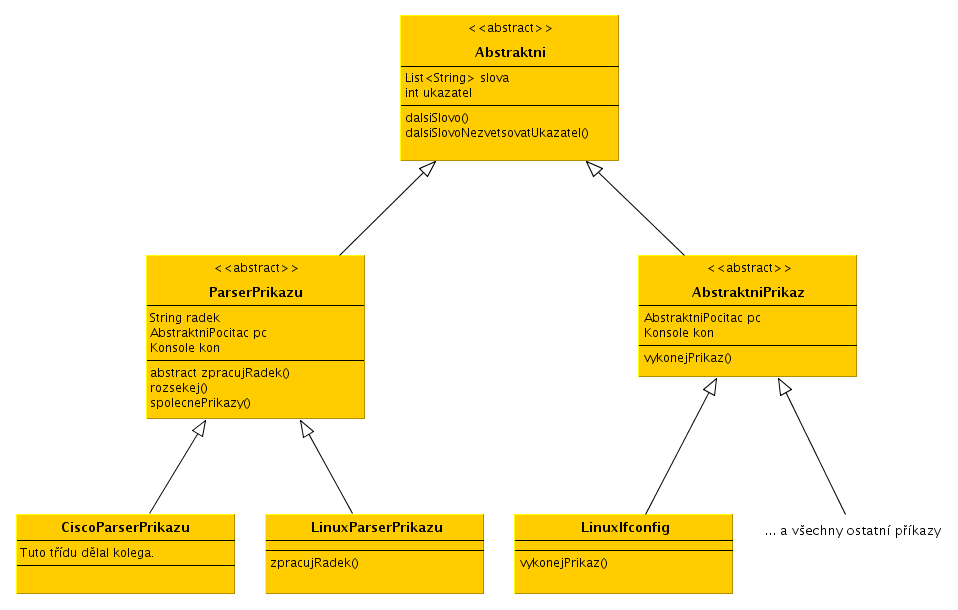
\includegraphics[width=14cm]{obrazky/prikazy}
\caption{Třídy pro zpracování příkazové řádky}
\label{obr_prikazy}
\end{center}
\end{figure}


\subsection{Třída Abstraktni}

Tato třída je abstraktním předkem všech ostatních tříd sloužících ke zpracování příkazů. Obsahuje pro parsování velmi důležitou metodu \verb|dalsiSlovo| a seznam slov jednoho řádku. Tato metoda postupně vrací jednotlivá slova ze seznamu. Je využívána skoro všemi potomky třídy \verb|Abstraktni| k parsování řádky. Dále jsou v této třídě různé statické metody využívané jednotlivými příkazy, například metoda \verb|zarovnej| na zarovnání slova v řetězci, metoda \verb|cekej|, která čeká zadaný počet milisekund a další.


\subsection{Třída ParserPrikazu}

Instanci jednoho z potomků této třídy, tedy \verb|LinuxParsePrikazu| nebo \verb|CiscoParsePrikazu|, si vytváří při své inicialisaci třída \verb|Konsole|, které slouží ke zpracování příkazové řádky. Jeho hlavní metodou je abstraktní \verb|zpracujRadek|, která je implementována v jeho potomcích a zpracovává jeden řádek, který uživatel do konzole napsal. K tomu používá metodu \verb|rozsekej|, jejímž autorem je můj kolega, která řádek zadaný jako \verb|String| \uv{rozseká} na jednotlivá slova a to tak, že jako oddělovače bere bílé znaky, tj. mezery a tabulátory. Rozsekaná slova pak uloží do seznamu řetězců \verb|slova|, který zdědila od svého předka třídy \verb|Abstraktni|. Třída \verb|LinuxParsePrikazu| podle prvního slova, které by mělo být názvempříkazu, vyvolá konstruktor třídy odpovídajícího příkazu. Nejdříve kontroluje, jestli příkaz není společným příkazem pro linuxový i ciscový počítač (příkaz \verb|uloz| nebo \verb|save|) a poté se snaží najít odpovídající linuxový příkaz. Jestliže uživatelem zadaný příkaz neexistuje nebo není implementován, vypíše \verb|LinuxParsePrikazu| uživateli řetězec \verb|bash: command not found| a zpracování řádku ukončí.


\subsection{Třída AbstraktniPrikaz}

Toto třída je potomkem třídy \verb|Abstraktni| a předkem tříd všech příkazů. Nemá žádnou důležitou metodu, ale parametry \verb|abstraktniPocitac pc| a \verb|konsole kon|, což jsou odkazy na počítač, na kterém příkaz probíhá a na konsoli, která ho vyvolala.



%------------------------------------------------------------------------------------------------------

\section{Společné znaky příkazů}

Příkazy, které jsem implementoval mají mnoho společného. Všechny jsou potomkem třídy \verb|AbstraktniPrikaz|, který je potomkem třídy \verb|Abstraktni|. Text, který byl uživatelem zadán, mají uložen v seznamu řetězců \verb|slova|. V konstruktoru příkazu je postupně voláno několik privátních metod. Metodou \verb|zparsujPrikaz| se nejprve parsuje vstup, většinou pomocí metody \verb|dalsiSlovo| zděděné ze třídy \verb|Abstraktni|. Při parsování se nastavují různé parametry příkazu, které uživatel zadal. Metoda \verb|zkontrolujPrikaz| kontroluje, jestli jsou nastaveny správné parametry a jestli byli zadány všechny. Potom metoda \verb|vykonejPrikaz| příkaz vykoná, to znamená, že změní konfiguraci počítače například u příkazu \verb|ifconfig|, nebo že provede nějakou jinou akci, například u příkazu \verb|ping| pošle několik paketů. Během těchto tří metod jsou ukládány případné chyby zadaného příkazu. Úplně nakonec příkaz vypíše případné chybové hlášení. Tento postup byl zvolen proto, že sladit správné pořadí vypisovaných chybových hlášení s postupem kontroly jednotlivých parametrů by bylo velmi náročné a nepřehledné. Příkazy svůj výstup posílají pomocí metod \verb|posli| a \verb|posliRade| třídy \verb|Konsole|.



%------------------------------------------------------------------------------------------------------

\section{Příkaz ifconfig}


\subsection{Teoretický úvod}

\verb|ifconfig| (zkratka \textbf{i}nter\textbf{f}ace \textbf{config}urator) je utilita unixových systémů, která slouží ke konfiguraci, kontrole  a vypsání informací o parametrech síťových rozhraní z příkazové řádky.\cite{wiki:ifconfig}. Pomocí této utility lze například vypsat parametry síťových rozhraní, nastavit IP nebo mac adresy, nastavit masky nebo \uv{nahodit} nebo \uv{schodit} rozhrani. Kromě toho, že \verb|ifconfig| nastavuje rozhraní, přidává nebo maže i záznamy v routovací tabulce, je-li to potřeba.


\subsection{Rozsah implementace v simulátoru}

V simulátoru musí \verb|ifconfig| umět nastavovat a mazat adresy IP a nastavovat masky. Samozřejmě také musí vypsovat nastavené parametry rozhraní. Změna mac adresy naproti tomu v našem simulátoru není vůbec potřeba. Parser příkazu \verb|ifconfig| je ale implementován i pro parametry \verb|add|, \verb|del|, \verb|up| a \verb|down|.

Zde uvádím příklady užití ifconfigu, které simulátor podporuje:
\begin{verbatim}
ifconfig eth0												vypíše parametry rozhraní eth0
ifconfig eth0 192.168.1.1								nastaví adresu na rozhraní eth0 
ifconfig eth0 10.0.0.1/8								nastaví adresu s maskou na rozhraní eth0
ifconfig eth0 10.0.0.2 netmask 255.255.0.0		nastaví adresu s maskou na rozhraní eth0
\end{verbatim}


\subsection{Analýza ifconfigu na skutečném počítači}\label{ifconfig_analysa}

Oproti jiným příkazům má \verb|ifconfig| pro simulaci jednu obrovskou nevýhodu: chybný parametr nezpůsobí ukončení příkazu, ale příkaz se dále provádí. Některé parametry je možné zadat vícekrát. Zjišťovat, jak se \verb|ifconfig| chová, proto bylo mnohem náročnější, než u ostatních příkazů. Zde popisuji výsledky této práce.

IP adresu je možné příkazu zadat vícekrát, všechno, co nelze zparsovat jinak se považuje za IP adresu. Je-li zadáno více adres, použije se adresa, které předchází první špatně adrese. Například:
\begin{verbatim}
ifconfig eth0 1.1.1.1 2.2.2.2 3.3.3.3			nastaví se poslední adresa, tj. 3.3.3.3

ifconfig eth0 1.1.1.1 blablabla 3.3.3.3		nastaví se adresa před první špatnou adresou, tj. 1.1.1.1
blablabla: unknown host
ifconfig: `--help' vypíše návod k použití.
\end{verbatim}
Adresu je možné zadat i s délkou prefixu za lomítkem. Je-li zadáno více adres a u jedné z nich je zadána délka prefixu, nastaví se taková maska, i když se tato adresa nepoužije. Například
\begin{verbatim}ifconfig eth0 1.1.1.1/1 2.2.2.2/2 3.3.3.3\end{verbatim}
nastaví adresu 3.3.3.3 s maskou 192.0.0.0, použije se tedy délka prefixu zadaná u druhé adresy. Adresa na rozhraní se maže nastavením adresy na 0.0.0.0.

Maska se nastavuje buď zadáním délky prefixu, jak je popsáno výše, nebo parametrem netmask. Zadá-li uživatel masku oběma způsoby, má přednost délka prefixu před parametrem netmask. Například
\begin{verbatim}ifconfig eth0 2.2.2.2/2 netmask 255.255.0.0\end{verbatim}
nastaví masku 192.0.0.0. Při změně IP adresy se automaticky mění i maska a to tak, že se maska dopočítá podle třídy IP adresy. Je-li tedy nejprve zadána maska parametrem netmask a teprve potom IP adresa, parametr netmask nemá žádnou účinnost. Například
\begin{verbatim}ifconfig eth0 netmask 255.255.255.0 1.1.1.1\end{verbatim}
nastaví adresu 1.1.1.1 s maskou 255.0.0.0.0, protože adresa 1.1.1.1 je třídy \verb|A|.

Příkaz \verb|ifconfig| promítá změny i do routovací tabulky. Změní-li se adresa na rozhraní, všecny záznamy na toto rozhraní se z tabulky vymažou. Při nastavení IP adresy se do routovací tabulky přidá záznam typu \verb|U| pro síť, ze které je tato adresa. Například při nastavení adresy
\begin{verbatim}ifconfig eth0 192.168.1.1/24\end{verbatim}
se do routovací tabulky přidá tento záznam:
\begin{verbatim}
Adresát         Brána           Maska           Přízn Metrik Odkaz  Užt Rozhraní
192.168.1.0     0.0.0.0         255.255.255.0   U     0      0        0 eth0
\end{verbatim}

Při zadání chybného vstupu se vykoná jen správná část příkazu a o těch špatných se vypíší chybová hlášení. Ty jsou vypisována v tomto pořadí:
\begin{enumerate}
\item špatný přepínač - příkaz se neprovádí
\item špatná adresa - žádná další chybová hlášení se nevypisují
\item špatné rozhraní
\item zakázaná adresa
\item špatné adresy parametrů \verb|add| nebo \verb|del|
\item chyba v gramatice
\end{enumerate}

Ostatními parametry se v tomto odstavci nezabývám, protože v simulátoru nejsou podporovány.


\subsection{Implementace v simulátoru}

V konstruktoru třídy \verb|LinuxIfconfig| jsou popoředě volány tyto metody: \verb|parsujPrikaz|, \verb|zkontrolujPrikaz|, \verb|vypisChybovyHlaseni| a \verb|vykonejPrikaz|. Parsování se v tomto příkaze neprovádí s využitím metody \verb|dalsiSlovo|, což by bylo dobré ještě upravit. Na rozdíl od skutečného ifconfigu se parsuje celý řádek, skutečný ifconfig parsování zastaví, když dojde ke špatnému přepínači nebo ke špatné adrese. Při parsování se parametry ukládají jako řetězce a ty jsou kontrolovány metodou \verb|zkontrolujPrikaz|. V tomto příkazu jsou chybová hlášení vypisována před již před samotným provedením příkazu a to v pořadí uvedeném v předchozím odstavci. Příkaz \verb|ifconfig| se metodou \verb|vykonejPrikaz| nakonec provede tak, aby to co nejvíce odpovídalo pravidlům uvedným v \ref{ifconfig_analysa}. Parametry \verb|add| a \verb|del| jsou v parsetu a kontrole implementovány, ale metoda \verb|vykonejPrikaz| je zatím ignoruje.


\subsection{Možnosti dalšího vylepšení}

Tento příkaz jsem implementoval jako první, kdy jsem s implementací příkazů ještě neměl zkušenosti, proto by se dal ještě v některých věcech vylepšit. Bylo by dobré přepsat metodu \verb|parsujPrikaz| tak, aby využívala metodu \verb|dalsiSlovo|, čímž by se zjednodušila, a dále ji předělat tak, aby se po špatné adrese již dále nic neparsovalo. Bylo by též dobré implementovat i parametry \verb|up| a \verb|down| s jejichž podporou se v analýze nepočítalo.


\subsection{Známé odchylky}

Zde uvádím známé odchylky implementace v simulátoru od skutečného příkazu na reálném počítači.\\
\verb|ifconfig eth0 netmask 255.0.0.0 2.2.2.2/2| ve skutečnosti spadne kvůli prefixu za adresou, v simulátoru to ale projde.\\
\verb|ifconfig eth0 blabla netmask 255.255.255.0| ve skutečnosti žádnou masku nenastaví, protože přestane parsovat už u blabla.\\
\verb|ifconfig eth0 netmask 255.255.255.0 10.0.0.1| by měl nastavit masku na 255.0.0.0, v simulátoru se nastaví 255.255.255.0



%------------------------------------------------------------------------------------------------------

\section{Příkaz route}

Příkaz route je utilita, která umožňuje administrátorovi vypisovat a měnit záznamy v routovací tabulce. Uvedu zde pár praktických příkladů:
\begin{verbatim}
route											vypíše routovací tabulku
Směrovací tabulka v jádru pro IP
Adresát         Brána           Maska           Přízn Metrik Odkaz  Užt Rozhraní
192.168.1.0     0.0.0.0         255.255.255.0   U     0      0        0 eth0
0.0.0.0         192.168.1.2     0.0.0.0         UG    0      0        0 eth0

route add -net 10.0.0.0/8 gw 192.168.1.3			Přidá záznam typu UG pro síť 10.0.0.0/8 na bránu 192.168.1.3
route del -net 10.0.0.0/8								Odebere minule přidaný záznam
\end{verbatim}


\subsection{Analýza příkazu route na skutečném počítači}

Oproti příkazu \verb|ifconfig| má příkaz route jasně definovanou gramatiku a při jakékoliv chybě v příkazu se příkaz neprovádí, proto byla implementace tohoto příkazu podstatně jednoduší. Příkaz má 2 hlavní akce, \verb|add| na přidávání záznamů a \verb|del| na jejich mazání. Nápověda uvádí ještě akci \verb|flush|, která ale není běžně podporována. Obě známé akce mají stejnou gramatiku. Parametr \verb|-net| přidá nebo odebere záznam pro síť, parametr \verb|-host| pro jednu adresu, tzn. záznam s maskou 255.255.255.255. Parametr \verb|gw| slouží k nastavení brány přidávanému nebo odebíranému záznamu, parametr \verb|dev| k nastavení rozhraní a parametr \verb|netmask| k nastavení masky přidávanému nebo odebíranému záznamu. Maska může být stejně jako v příkazu \verb|ifconfig| zadána parametrem \verb|netmask| nebo pomocí délky prefixu za lomítkem, např. \verb|10.0.0.0/16|. Při použití parametru \verb|-net| musí být vždy maska nějakým způsobem zadána. Adresát, tzn. parametr \verb|-net| nebo \verb|-host| musí být vždy prvním parametrem akce, na pořadí dalších parametrů již nezáleží. Parametry \verb|-host| a \verb|dev| není nutno psát. Žádný parametr nemůže být zadán vícektrát. Akce \verb|add| vyžaduje aspoň jeden z parametrů \verb|gw| nebo \verb|dev|. Narazí-li se při provádění přikazu na chybu, je vypsáno chybové hlášení a příkaz se ukončí, aniž by se vykonala jeho správná část.


\subsection{Implementace v simulátoru}

Implementoval jsem parametry \verb|-host|, \verb|-net|, \verb|netmask|, \verb|dev| a \verb|gw|. Parser tohoto příkazu je psán za pomocí metody \verb|dalsiSlovo| celkem přehledně, každý parametr se parsuje vlastní metodou. Parser též kontroluje správnost příkazu, vypisuje chybová hlášení a nastavuje parametry. Metoda \verb|vykonejPrikaz| upravuje nebo vypisuje routovací tabulku příslušného počítače.


\subsection{Odchylky}

Akce \verb|flush| sice není na normální počítači implementována, avšak v simulátoru jsem ji implementoval s tím, že simulátor vypíše varovné hlášení:
\begin{verbatim}
linux1:~# route flush
psi simulator: Flush normalne neni podporovano, ale routa se v simulatoru smaze.
Spravny prikaz je: "ip route flush all"
\end{verbatim}



%------------------------------------------------------------------------------------------------------

\section{Příkaz ping}

Tento příkaz posílá ICMP pakety typu \verb|request| (žádost o odpověď) a přijímá pakety typu \verb|ICMP reply|. Uživateli umožňuje prověřit funkčnost spojení mezi dvěma počítači v síti.


\subsection{Analýza skutečného pingu}

Příkazu musí uživatel zada cílovou adresu, na kterou se chce \uv{dopingnout}. Dále je možné použít několik přepínačů. Přepínačem \verb|-c| si uživael určí, kolik paketů chce poslat, není-li tento parametr zadán, posílaji se pakety pořád, dokud uživatel příkaz nezastací \verb|Ctrl+C|. Parametrem \verb|-s| je možne specifikovat velikost posílaného paketu, parametrem \verb|-i| se specifikuje interval mezi odesláním dvou paketů. Parametrem \verb|-t| je možné zadat \verb|ttl| odchozích paketů. Parametr \verb|-b| umožňuje posílat \verb|icmp request| na broadcastovou adresu a parametr \verb|-q| potlačuje výstup příkazu. Parametr \verb|-b| není v simulátoru podporován. Například příkaz:
\begin{verbatim}
ping -c10 -i 0.1 -s1000 -t 23  192.168.2.2
\end{verbatim}
pošle 10 paketů v intervalu 0,1 sekundy o velikosti 1000 bytů s ttl 23 na adresu 192.168.2.2. Na pořadí parametrů nezáleží, jejich hodnoty můžou být uvedeny bez mezery i s ní. U tohoto příkazu lze zadat přepínače i po IP adrese.


\subsection{Implementace v simulátoru}

Virtuální pakety, které si předávají virtuální počítače našeho simulátoru, si nesou i odkaz na příkaz, který je vyvolal. To proto, aby když počítači dorazí \verb|icmp reply| počítač věděl, který příkaz je původcem tohoto paketu. Proto všechny příkazy, které v našem simulátoru posílají pakety jsou potomkem abstraktní třídy \verb|AbstraktniPing| jejíž abstraktní metodu \verb|zpracujPaket| volá přímo metoda počítače, který paket přijala. Tato třída má také metodu \verb|aktualizujStatistiky|, která spočítá konečné statistiky příkazu.

Parser tohoto příkazu je podobný jako v ostatních příkazech, pomocí metody \verb|dalsiSlovo| se parsují jednotlivé parametry. Příkaz nemá zvláštní metodu pro kontrolu pro výpis chybových hlášení. Metoda \verb|vykonejPrikaz| posílá pomocí metody \verb|posliIcmpRequest| třídy \verb|AbstraktniPocitac| jednotlivé pakety a pak je metodou \verb|zpracujPaket| zpracovává.

Čas odezvy vypisovaný tímto příkazem není skutečný, ale každý počítač procházejícímu paketu do parametru čas přičte náhodně vygenerovanou hodnotu a to tak, aby hodnoty byly přibližně stejné, jako jsou v laboratořích předmětu PSI.


\subsection{Odchylky v implementaci}

Protože program telnet, přes který se budou uživatelé simulátoru přihlašovat k počítačům neumí přeposílat \verb|Ctrl+C|, musím v našem simulátoru mít nastavený výchozí počet odesílaných paketů na 4, aby uživatel tento příkaz mohl nějak zastavit. Toto je velký rozdíl oproti skutečnému pingu na linuxu, ale neměl jsem jinou možnost.

Parametr \verb|-i|, kterým se nastavuje interval mezi odesláním dvou paketů, se musí v simulátoru zadat tak, aby mezi \verb|-i| a hodnoutou byla mezera. Není tedy možné napsat \verb|-i0.5|.

V simulátoru musí být oproti skutečnosti přepínače napsané před adresou. Ve skutečnosti to není nutné. Tento nedostatek ještě opravím.



%------------------------------------------------------------------------------------------------------

\section{Příkaz traceroute}

Program traceroute slouží k analýze počítačové sítě. Vypisuje uzly (resp. směrovače) na cestě datagramů od zdroje až k zadanému cíli. Uzly jsou zjišťovány pomocí snížení hodnoty TTL v hlavičce datagramů.\cite{wiki:traceroute}.


\subsection{Popis činnosti}

Příkaz posílá pakety ICMP request na cílovou adresu, kterým postupně zvyšuje \verb|ttl|, dokud nedojte od cílového počítače paket ICMP reply. Počítače, které paket nemohou dále poslat, protože mu \verb|ttl| vypršelo, posílají zdrojovému počítači zprávu ICMP time exceeded. Podle těchto zpráv příkaz zjistí, kterými uzly procházejí pakety k cílové adrese.

Příklad výpisu příkazu:
\begin{verbatim}
neiss: ~/smazat$ traceroute -n 89.190.94.58
traceroute to 89.190.94.58 (89.190.94.58), 30 hops max, 60 byte packets
 1  192.168.1.20  0.833 ms  1.257 ms  1.691 ms
 2  10.4.71.1  66.723 ms  67.245 ms  69.029 ms
 3  89.190.94.2  69.648 ms  70.088 ms  70.422 ms
 4  89.190.94.58  70.893 ms  71.261 ms  74.190 ms
\end{verbatim}


\subsection{Implementace}

Třída příkazu \verb|traceroute| dědí ze třídy \verb|AbstraktniPing|, aby odkaz na ní mohl být posílán spolu s paketem. Příkaz nemá prakticky žádný parser, jediná povolená syntaxe tohoto příkazu je \verb|traceroute <adresa>|. Pokud uživatel zadá neodpovídající vstup, vypíše se mu hlášení, jaká je jediná povolená syntaxe. Příkaz funguje na stejném principu jako příkaz skutečný, jak je popsáno v předchozím odstavci.



%------------------------------------------------------------------------------------------------------

\section{Příkaz exit}

Příkaz \verb|exit| je jedinou korektní možností ukončení relace. Zavolá metodu \verb|ukonciSpojeni| třídy \verb|Konsole|, čímž ukončí běh její metody \verb|run| a tak se spojení ukončí.



%------------------------------------------------------------------------------------------------------

\section{Příkaz ip}

Příkaz \verb|ip| je plnohodnotnou náhradou za příkazy \verb|ifconfig|, \verb|route|, \verb|arp|. Umožňuje však i pokrocilejší správu síťových nastavení\cite{prikaz_ip}. Já jsem z tohoto příkazu ve svém simulátoru implementoval jeho dva základní podpříkazy \verb|addr| pro nastavení parametrů rozhraní a \verb|route| pro manipulaci se směrovací tabulkou. 


\subsection{Implementace}

Příkaz \verb|ip| je implementován třídou \verb|LinuxIp|. Jeho podpříkazy \verb|addr| a \verb|route| ale byly implementovány samostatně, to znamená, že jsem pro každý podpříkaz vytvořil vlastní třídu. Třída \verb|LinuxIp| parsuje přepínače a jméno podpříkazu. Je-li napsaný podpříkaz podporován, spustí odpovídající třídu, která pak funguje stejně jako samostatný příkaz. Není-li podporován, vypíše o tom hlášení. 

Parsování příkazu \verb|ip| má jednu zvláštnost. Není totiž nutné, aby uživatel psal všechny terminály, ale místo některých lze napsat třeba jen první písmeno, které terminál jednoznačně určuje. Tak například místo řádku
\begin{verbatim}
ip addr add 1.1.1.1 dev eth0
\end{verbatim}
lze jednoduše napsat
\begin{verbatim}
ip a a 1.1.1.1 dev eth0
\end{verbatim}
Tuto možnost podporuji i v simulátoru.


\subsection{Podpříkaz addr}

\subsubsection{Analýza podpříkazu}

Tento příkaz slouží především k přidávání a mazání adres na rozhraní. Má 4 akce: \verb|add| na přidání adres, \verb|del| na odebrání adresy, \verb|flush| na smazání všech adres na rozraní a \verb|show| na vypsání nastavených adres. Akce show je výchozí, není ji tedy nutno psát. Existující adresu na rozhraní není možno tímto příkazem změnit, je nutné starou IP odstranit a novou přidat. 

\subsubsection{Implementace}

Tento příkaz je prováděn klasicky metodami \verb|parsujPrikaz|, \verb|zkontrolujPrikaz|, \verb|vykonejPrikaz| a \verb|vypisChybovyHlaseni|. Parser má pro každý parametr vlastní parsovací metodu. Kontrolovací metoda kontroluje zadané parametry podle akce, protože u každé akce mohou být jiné parametry.

\subsubsection{Známé odchylky}

V simulátoru není možné nastavit více adres a jednom rozhraní, když se o to uživatel snaží, vypíše mu simulátor varovné hlášení:
\begin{verbatim}
linux2:~# ip a a 1.1.1.1/22 dev eth0
psi simulator: Simulator nepodporuje vice adres na jednom rozhrani. Na rozhrani eth0 je jiz adresa 1.1.11.1/23. Odstrante ji prikazem flush nebo del.
\end{verbatim}

Akcím \verb|flush| a \verb|show| je možné zadat selektrory na vybrání mazaných nebo zobrazovaných adres. Ty nejsou v příkazu podporovány.

Na počítačích v laboratoři PSI projde příkaz
\begin{verbatim}
ip a a 600.0.0.1
\end{verbatim}
tuto možnost však v simulátoru nepodporuji.


\subsection{Podpříkaz route}

\subsubsection{Analýza}

Příkaz \verb|ip route| je alternativou k příkazu \verb|route|, funguje prakticky stejně, ale má jinou, o něco jednoduší gramatiku. Na rozdíl od příkazu \verb|route| neumožňuje přidat do routovací tabulky záznam na adresáta, který již v tabulce je. Má 5 akcí: \verb|add| a \verb|del| na přidávání a mazání záznamů, \verb|show| a \verb|flush| na vypsání a mazání všech záznamů a akci get, které se zadá cílová IP adresa a příkaz vypíše záznam ze směrovací tabulky, podle kterého by se směrovalo k této adrese. Všechny akce mají prakticky stejnou gramatiku, jen u akce \verb|get| není povoleno zadat parametr \verb|via|, což je obdoba parametru \verb|gw| z příkazu \verb|route|.

\subsubsection{Implementace v simulátoru a její odchylky od skutečnosti}

Způsob vykonávání tohoto příkazu je stejný jako u podpříkazu \verb|addr|. Část metody \verb|vykonejPrikaz| jsem mohl přejmout z příkazu \verb|route|. V simulátoru nejsou podporovány selektory u akcí \verb|show| a \verb|flush|, u akce \verb|get| není podporován parametr \verb|dev|, o čemž se případně vypíše varovné hlášení.



%------------------------------------------------------------------------------------------------------

\section{Příkaz iptables}

Příkaz \verb|iptables| je utilita, která umožňuje nastavovat paketový filtr jádro operačního systému Linux. V simulátoru implementuji jen malou část rozsáhlého příkazu, která slouží k nastavování překladu adres.

Simulátor na linuxovém počítači podporuje jen tzv. statický NAT, který překládá všechny pakety odcházející přes rozhraní na jednu veřejnou IP adresu. V této práci se překladem adres nezabývám, tuto problematiku řešil především můj kolega, více informací je v jeho bakalářské práci. 


\subsection{Implementace}

Příkaz je implementován k tomu, aby pomocí něj bylo možné nastavit statický překlad adres, vypsat jeho nastavení a vymazat ho, což se provádí například těmito příkazy:
\begin{verbatim}
iptables -t nat -I POSTORUTING -o eth2 -j MASQUERADE		nastavení
iptables -t nat -L													vypsání
iptables -t nat -D POSTROUTING 1									smazání

\end{verbatim}
Parser je však implementován mnohem robustněji a umožňuje v budoucnosti přidat další možnosti nastavení. Oproti reálnému počítači není v našem simulátoru dovoleno nastavovat více pravidel pro překlad adres.




\chapter{Uživatelské testování}

Uživatelské testování prováděl tester za přítomnosti mé a mého kolegy z~týmu. Jeho hlavním účelem bylo najít chyby v~programu, na které jsem sám nepřišel. V~této kapitole popisuji pouze testování těch částí systému, které jsem sám programoval. Testování částí, které dělal kolega, zde nepopisuji.



%----------------------------------------------------------------------------------------------------------

% uziv. zkusil zmenit MAC adresu - chyba
% ifconfig --help vypsal chybu, at uzivatel zkusi ifconfig --help
% ping -c 4 192.168.1.1 - chyba -mezera mezi 'c' a 4
% ping IP prepinace - nefunguje
% man route nefunguje
% route -h a --help a --version nefunguje
% prepsat vypisy z Cj do Aj 
% echo 1 > ip_forward - ma tam byt jen /proc/sys/net/..


\section{Průběh testování}


\subsection{Spuštění aplikace}

Prvním úkolem testera bylo aplikaci spustit a zjistit, jak se s~ní zachází. Toto činilo uživateli menší problémy, protože chybová hlášení vyhazovaná simulátorem nebyla dost jasná na to, aby uživatel pochopil, jak se má chyb vyvarovat. Spouštění aplikace je práce mého kolegy a ten chyby opravil.


\subsection{Práce s~aplikací}

Tester měl za úkol zkonfigurovat síť z obrázku \ref{obr_testovani}. Během konfigurace přišel na chyby, které zde popisuji, a zároveň také popisuji, jak byly opraveny.

% testovací síť
\begin{figure}[h]
\begin{center}
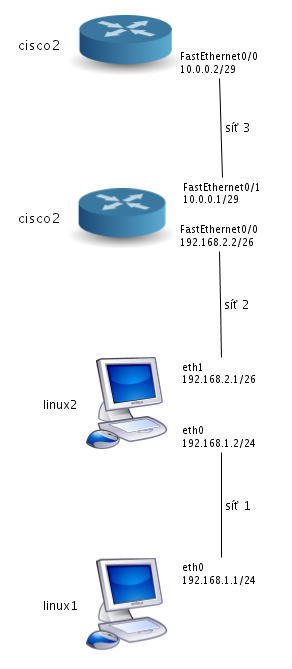
\includegraphics[width=5cm]{obrazky/testovani}
\caption{Testovací síť, kterou tester konfiguroval}
\label{obr_testovani}
\end{center}
\end{figure}

\subsubsection{Výpisy}

Hlášení o~běhu simulátoru, která jsou vypisována na standardní výstup, se testerovi zdála velmi nepřehledná. Výpisy o~tom, co server posílá jednotlivým klientům a co klienti posílají serveru, jsou pro uživatele nadbytečné a proto byly zrušeny. Ponechány byly jen výpisy o~přihlášení klienta a o~průchodu paketu, které byly testerovi užitečné pro diagnostiku sítě.

\subsubsection{Příkaz ifconfig}

Tester zkoušel změnit mac adresu rozhraní, což simulátor nepodporuje. Přidal jsem příkaz \verb|help|, který popisuje, jaké varianty příkazů jsou podporovány.

Tester zkoušel příkaz \verb|ifconfig --help|, který nefunguje. Chybu jsem opravil.

\subsubsection{Manuálové stránky}

Tester zkusil zadat \verb|man route|, přičemž simulátor vypsal, že příkaz neexistuje. Dodělal jsem příkaz \verb|man|, který vypíše, že manuálové stránky nejsou implementovány a doporučí uživateli příkaz \verb|help|.

\subsubsection{Příkaz ping}

Uživatel zadal příkaz \verb|ping 192.168.1.1 -c5|. Zjistil, že parametr \verb|-c| je ignorován, protože parser parsuje jen parametry před adresou. Parser jsem z důvodu veliké časové tísně zatím nestihl opravit. Chyba je zmíněna přímo u popisu tohoto příkazu a bude opravena.

\subsubsection{Soubor ipforward}

Z důvodů snazšího testování jsem měl na soubor \verb|/proc/sys/net/ipv4/ip_forward| nastaven alias \verb|ip_forward|, který jsem zapomněl odstranit. Alias již byl odstraněn.

\subsubsection{Příkaz route}

Tester zkoušel příkaz \verb|route --help|, který nefunguje. Do parseru jsem přidal parsování tohoto přepínače.



%----------------------------------------------------------------------------------------------------------

\section{Závěr}

V aplikaci bylo nalezeno několik, spíše drobnějších chyb především v parsování příkazů. Některé chyby již byly opraveny, některé teprve opravím a jistě existují chyby, zvláště v parserech, které ještě nebyly nalezeny. Ty budu muset opravit, až na ně uživatelé, budou-li kdy nějací, přijdou.

V simulátoru nebyly nalezeny žádné vážnější chyby v jeho datových strukturách a ve virtuální síti. Nebyly nalezeny ani žádné chyby, které by způsobovaly pád naší aplikace.




%*****************************************************************************
% Seznam literatury je v samostatnem souboru reference.bib. Ten
% upravte dle vlastnich potreb, potom zpracujte (a do textu
% zapracujte) pomoci prikazu bibtex a nasledne pdflatex (nebo
% latex). Druhy z nich alespon 2x, aby se poresily odkazy.

% originally following specification for bibliography formating was used
%\bibliographystyle{abbrv}

% Here is an improvment by Petr Dlouhy (April 2010).
% It is mainly for supervisors who expect Czech fomrating rules for references
% Additional feature is live url addresses to sources from your pdf file
% It requires the file csplainnat.bst (included in this sample zipfile).

\bibliographystyle{csplainnat}

%bibliographystyle{plain}
%\bibliographystyle{psc}
{
%JZ: 11.12.2008 Kdo chce mit v techto ukazkovych odkazech take odkaz na CSTeX:
\def\CS{$\cal C\kern-0.1667em\lower.5ex\hbox{$\cal S$}\kern-0.075em $}
\bibliography{reference}
}

% M. Dušek radi:
%\bibliographystyle{alpha}
% kdy citace ma tvar [AutorRok] (napriklad [Cook97]). Sice to asi neni  podle ceske normy (BTW BibTeX stejne neodpovida ceske norme), ale je to nejprehlednejsi.
% 3.5.2009 JZ polemizuje: BibTeX neobvinujte, napiste a poskytnete nam styl (.bst) splnujici citacni normu CSN/ISO.

%*****************************************************************************
%*****************************************************************************
\appendix

%*****************************************************************************
\chapter{Seznam použitých zkratek}

\begin{description}
\item[2D] Two-Dimensional
\item[ABN] Abstract Boolean Networks
\item[ASIC] Application-Specific Integrated Circuit
\end{description}
\vdots

%*****************************************************************************
\chapter{Instalační a uživatelská příručka}
\textbf{\large Tato příloha velmi žádoucí zejména u softwarových implementačních prací.}

%*****************************************************************************
\chapter{Obsah přiloženého CD}
\textbf{\large Tato příloha je povinná pro každou práci. Každá práce musí totiž obsahovat přiložené CD. Viz dále.}

Může vypadat například takto. Váš seznam samozřejmě bude odpovídat typu vaší práce. (viz \cite{infodp}):

\begin{figure}[h]
\begin{center}
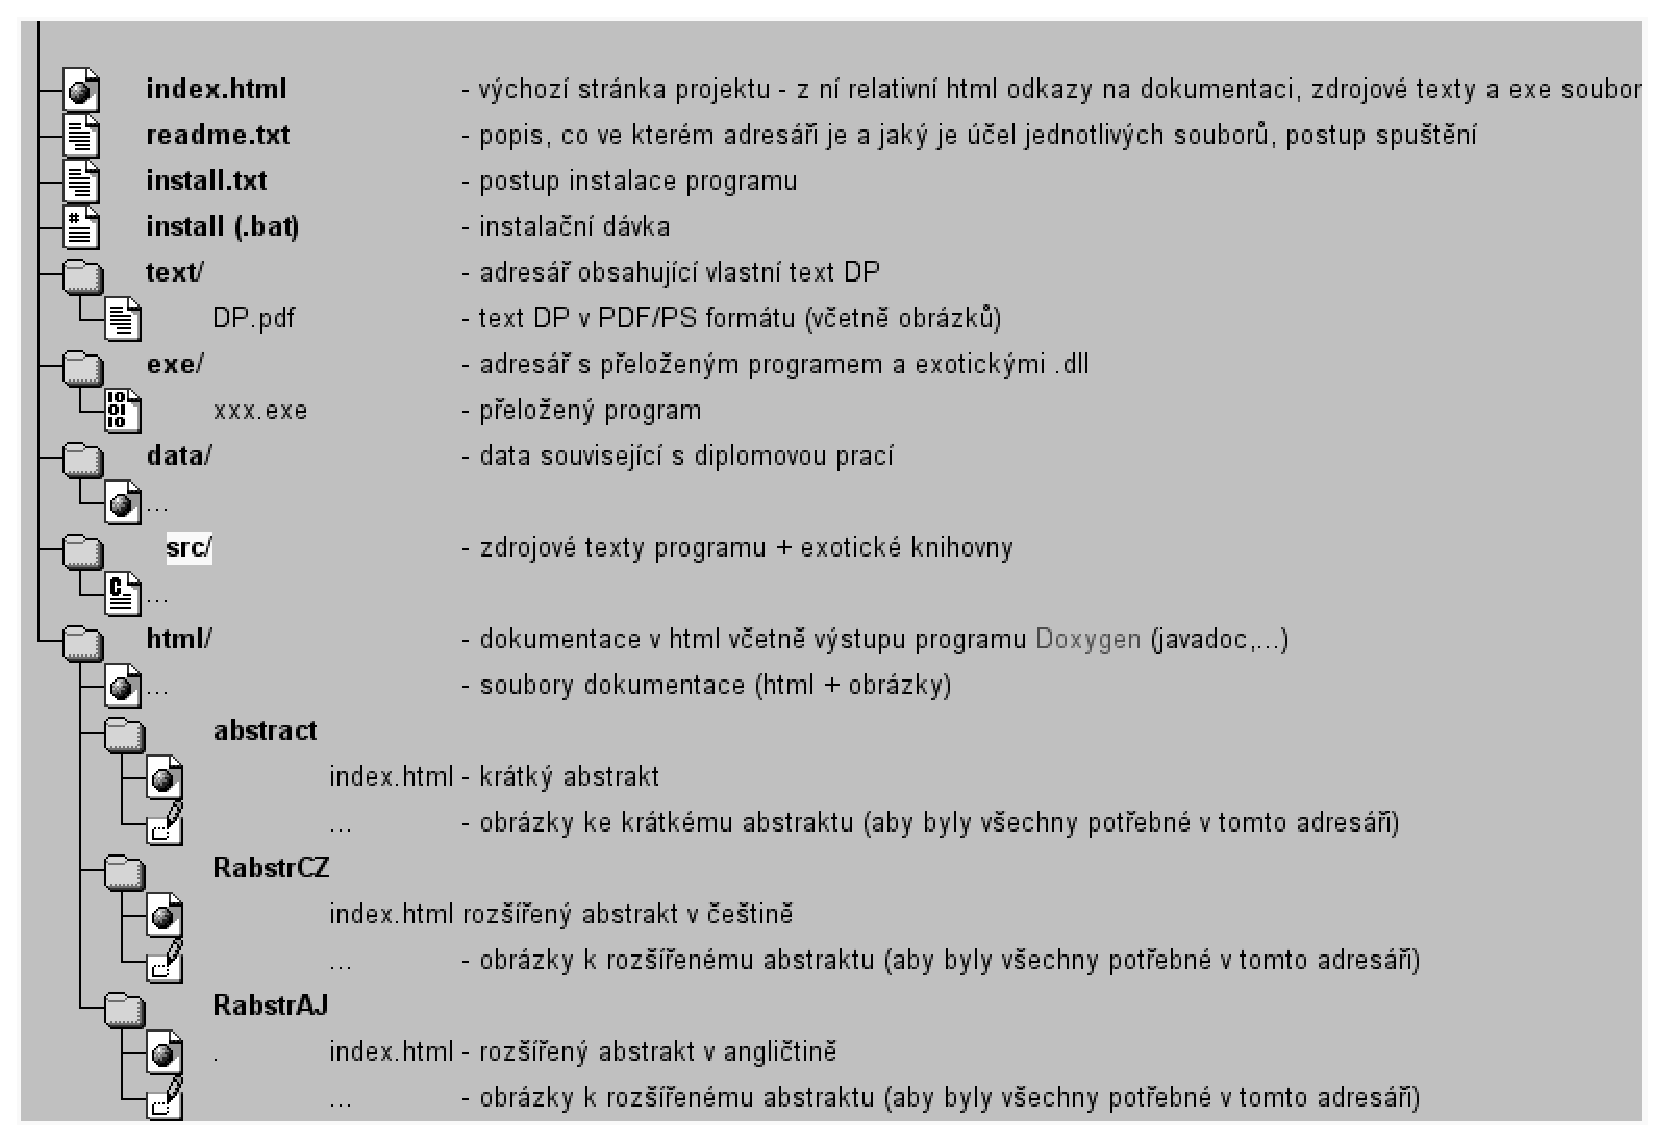
\includegraphics[width=14cm]{figures/seznamcd}
\caption{Seznam přiloženého CD --- příklad}
\label{fig:seznamcd}
\end{center}
\end{figure}

Na GNU/Linuxu si strukturu přiloženého CD můžete snadno vyrobit příkazem:\\ 
\verb|$ tree . >tree.txt|\\
Ve vzniklém souboru pak stačí pouze doplnit komentáře.

Z \textbf{README.TXT} (případne index.html apod.)  musí být rovněž zřejmé, jak programy instalovat, spouštět a jaké požadavky mají tyto programy na hardware.

Adresář \textbf{text}  musí obsahovat soubor s vlastním textem práce v PDF nebo PS formátu, který bude později použit pro prezentaci diplomové práce na WWW.

\end{document}
